% !TeX program = lualatex
% !BIB program = biber
\documentclass[11pt,a4paper]{article}

\usepackage{fontspec}
\usepackage{csquotes}
\usepackage{geometry}
\geometry{margin=2.5cm}
\usepackage{booktabs}
\usepackage{graphicx}
\usepackage{amsmath}
\usepackage{caption}
\usepackage{subcaption}
\usepackage{threeparttable}
\usepackage{array}
\usepackage[backend=biber,style=authoryear,maxcitenames=2,maxbibnames=99]{biblatex}
\addbibresource{referencias.bib}
\usepackage[colorlinks=true,linkcolor=blue,citecolor=blue,urlcolor=blue]{hyperref}
\usepackage{orcidlink}

\captionsetup{font=small,labelfont=bf}
\setlength{\parskip}{0.35em}
\setlength{\parindent}{0pt}
\setlength{\emergencystretch}{3em}

\title{\textbf{Temporal Disaggregation and the Illusion of Fiscal Leakage: Evidence from Timor-Leste}}
\author{
  \begin{tabular}{c@{\hspace{2em}}c}
    Emerson López\,\raisebox{0.25em}{\scalebox{1.25}{\orcidlink{0009-0009-6423-2883}}} & Julio Gomez\\
    \small\href{mailto:emerson.zeledon.ni@gmail.com}{\texttt{emerson.zeledon.ni@gmail.com}} &
  \end{tabular}
}
\date{\today}

\begin{document}
\maketitle

\begin{abstract}
\noindent
Data-limited economies often disaggregate annual national accounts before estimating quarterly fiscal models. This paper shows that the disaggregation step can manufacture the central result. Using official quarterly national accounts for Timor-Leste from 2014Q1 to 2023Q4, a Bayesian VAR and local projections find no robust evidence that a government expenditure shock produces a large or persistent increase in imports. The estimated import response is below 0.4\% at all horizons, while the response of non-oil GDP is small and short-lived. In contrast, the same models estimated on a 2002--2023 sample built by Denton--Cholette temporal disaggregation generate a large, precisely estimated import response, peaking near 2\% in the BVAR and 24\% in local projections. The difference is not the estimator, the prior, or the identification: it is how the data are constructed. Interpolation smooths the fiscal and outcome series and induces a mechanical comovement that the VAR attributes to fiscal transmission. A hybrid model that combines a smooth, interpolated government series with official outcomes does not reproduce the leakage. The results caution against using interpolated quarterly data to identify fiscal leakage in small open economies.
\end{abstract}

\section{Introduction}
\label{sec:introduction}

Timor-Leste is a small, open, petroleum-rich economy with a short macroeconomic history. Government expenditure finances state-building, infrastructure, and a large share of domestic absorption, while the productive base remains narrow. A central policy question is therefore whether fiscal expansion supports domestic non-oil activity or leaks abroad through imports. Because the country's national accounts are available at annual frequency for most of the sample, earlier versions of this analysis relied on temporally disaggregated quarterly data to estimate dynamic fiscal models.

This paper revisits that question with official quarterly data. The Instituto Nacional de Estatística (INETL) publishes quarterly GDP by expenditure from 2014 onwards. We use these data to estimate a quarterly Bayesian VAR (BVAR) and local projections (LP) for 2014Q1--2023Q4, and we compare the results with those obtained from a long 2002--2023 sample constructed by univariate Denton--Cholette disaggregation. The comparison is designed to separate the effect of the estimator from the effect of the data.

The main finding is that the strong leakage result is not robust. In the official sample, a three-variable BVAR with government expenditure, imports, and non-oil GDP is stable and estimates an import response below 0.1\% at short horizons and no persistent increase. Local projections confirm that the official import response is small, between $-0.4\%$ and $0.4\%$ depending on the horizon, and economically negligible relative to the long-sample estimates. Non-oil GDP shows a small impact response in the BVAR but no robust positive response in the LP. The five-variable official BVAR, which adds the CPI and private credit, is unstable because the short sample cannot support the additional dynamics; this instability is itself informative about the limits of the official sample.

In the long interpolated sample, the same three-variable BVAR is stable and estimates a significant import response that rises to about 2.1\% after six to seven quarters. The LP estimates are larger, peaking near 24\% after two to three quarters. The long-sample results reproduce the earlier finding: imports respond earlier and more strongly than non-oil GDP. The contrast between the two samples is stark, and it survives alternative orderings, seasonal adjustment choices, and a hybrid specification that uses a broader interpolated government series with official outcomes.

The contribution is threefold. First, the paper provides BVAR and LP estimates for Timor-Leste based on official quarterly national accounts, rather than interpolated annual data. Second, it documents a methodological pitfall: temporal disaggregation can generate spurious fiscal transmission because it imposes smoothness and a common annual benchmark on all series. Third, it offers a practical warning for policy analysis in data-limited economies: estimates of fiscal leakage based on interpolated quarterly data should be treated with caution, and the result should be tested against official high-frequency data whenever available.

The remainder of the paper is organized as follows. Section~\ref{sec:literature} reviews the literature. Section~\ref{sec:data} describes the data and the construction of the long sample. Section~\ref{sec:method} presents the empirical strategy. Section~\ref{sec:results} reports the results and robustness checks. Section~\ref{sec:conclusion} concludes.

\section{Literature}
\label{sec:literature}

The macroeconomic effects of fiscal policy have been extensively studied, but consensus on the size of fiscal multipliers remains elusive, especially in developing and resource-rich economies. \textcite{blanchard2002} introduced the structural VAR approach to identify government spending shocks and showed that spending increases typically raise output. \textcite{mountford2009} used sign restrictions to show that fiscal effects depend on the type of shock and the state of the economy. For small open economies, the literature emphasizes that multipliers tend to be smaller because part of the stimulus is absorbed by imports. \textcite{ilzetzki2013} find lower multipliers in economies with more open trade regimes and more flexible exchange rates. Resource-rich economies face additional challenges: commodity-price volatility and Dutch-disease pressures complicate the conduct of fiscal policy \parencite{frankel2012}.

Vector autoregressions are the standard tool for dynamic multivariate analysis, but short time series make unrestricted OLS estimates unreliable. Bayesian VARs, introduced to macroeconomics by \textcite{litterman1986} and refined by \textcite{giannone2015}, impose prior beliefs that shrink the parameter space and can produce stable responses even with limited observations. The \texttt{BVAR} package of \textcite{bvar2021} implements hierarchical prior selection for these models.

A separate literature addresses the construction of high-frequency data from annual benchmarks. \textcite{denton1971} proposed a quadratic minimization method, extended by \textcite{cholette1984}; \textcite{saxsteiner2013} and the \texttt{tempdisagg} package implement these methods in R. Temporal disaggregation is widely used in data-poor settings, but it is not a source of new information: it distributes an annual total using a smoothness criterion or a related indicator. The resulting quarterly series are mechanically smooth and share the annual benchmark with the other disaggregated variables. This paper shows that such shared smoothness can be mistaken for dynamic causal transmission.

Studies of fiscal policy in Timor-Leste are scarce, but the available estimates point to small multipliers. \textcite{worldbank2021} estimates an impact multiplier of 0.17 and a cumulative multiplier of 0.08 using a quarterly SVAR for 2010--2019 with real quarterly data. \textcite{imf2024} reports multipliers of 0.1--0.2, attributing the small size to the low quality and high import content of public spending. These estimates are consistent with the small official-data responses documented below, and they are difficult to reconcile with the large leakage implied by the interpolated sample. This paper contributes by combining official quarterly data with a transparent comparison to the interpolated sample, and by showing that the difference between the two is large enough to change the substantive conclusion.

\section{Data}
\label{sec:data}

\subsection{Official quarterly data}
\label{sec:official}

The baseline data are the official quarterly national accounts published by INETL for 2004--2023 \parencite{inetl2023}. We use the expenditure table (Table~7.1) at constant 2015 prices for 2014Q1--2023Q4, the period for which quarterly observations are available. The sample contains 40 quarters. The variables are general government final consumption expenditure, non-oil GDP by expenditure, and imports of goods and services. The consumer price index is obtained from the monthly DNE series and averaged to quarterly frequency \parencite{dne_cpi}. Credit to the private sector is the BCTL monetary survey series, measured at the end of each quarter \parencite{bctl2024}.

The official series are seasonally adjusted with X-13ARIMA-SEATS before estimation. The baseline uses the seasonally adjusted data; an unadjusted specification with quarterly dummies is reported as a robustness check. Table~\ref{tab:variables} summarizes the variables and sources.

\begin{table}[htbp]
\centering
\small
\caption{Variables, sources, and samples}
\label{tab:variables}
\resizebox{\textwidth}{!}{%
\begin{tabular}{@{}llll@{}}
\toprule
Variable & Interpretation & Official baseline (2014--2023) & Long-sample comparison (2002--2023) \\
\midrule
\texttt{ln\_gov\_exp} & Government expenditure & General Government FCE, INETL & ADB government expenditure, interpolated \\
\texttt{ln\_gdp\_non} & Real non-oil GDP & GDP by expenditure, INETL & ADB non-oil GDP, interpolated \\
\texttt{ln\_imports} & Real imports & Imports of goods and services, INETL & ADB imports, interpolated \\
\texttt{ln\_cpi} & Consumer price index & DNE monthly CPI, quarterly average & DNE/ADB CPI \\
\texttt{ln\_credit} & Private credit & BCTL domestic credit, end-of-quarter & ADB private credit \\
\bottomrule
\end{tabular}}
\par\vspace{0.3em}
\begin{minipage}{0.95\textwidth}
\footnotesize\textit{Note:} All real variables are in millions of USD at constant 2015 prices. The official sample is 2014Q1--2023Q4 (40 observations); the long sample is 2002Q1--2023Q4 (88 observations). The baseline BVAR uses government expenditure, imports, and non-oil GDP; the CPI and credit enter the five-variable robustness models.
\end{minipage}
\end{table}

\subsection{Data validation and source differences}
\label{sec:validation}

The official quarterly GDP and import series aggregate almost exactly to the annual ADB series \parencite{adb2025}. Over 2014--2023, the largest absolute difference between the sum of the four quarterly observations and the annual figure is 0.85 million USD for GDP (2016) and 1.10 million USD for imports (2021). These differences are negligible relative to annual levels of about 1,500--1,650 million USD for GDP and 730--980 million USD for imports.

Two source differences require attention. First, the official General Government FCE is systematically lower than the ADB government expenditure series, by 180 million USD in 2014 and 124 million USD in 2023. The official measure is a national-accounts component and is narrower than the ADB aggregate, which may include other public spending. Second, the BCTL domestic credit series matches the ADB private credit series until 2017, but is about 50 million USD lower from 2018 to 2022 and 6 million USD lower in 2023. The break is consistent with a definitional change in the monetary survey. We use the BCTL series for the official sample and report the discrepancy rather than forcing the two sources to match. Table~\ref{tab:validation} summarizes the comparison.

\begin{table}[htbp]
\centering
\small
\caption{Comparison of official quarterly and annual ADB series, 2014--2023}
\label{tab:validation}
\resizebox{\textwidth}{!}{%
\begin{tabular}{@{}lll@{}}
\toprule
Series & Comparison & Result \\
\midrule
GDP & Sum of quarters vs annual ADB & Max.\ absolute difference 0.85 (2016) \\
Imports & Sum of quarters vs annual ADB & Max.\ absolute difference 1.10 (2021) \\
Government FCE & Sum of quarters vs ADB government expenditure & 124--180 million USD lower every year \\
Private credit & Q4 vs annual ADB & About 50 million USD lower in 2018--2022 \\
\bottomrule
\end{tabular}}
\par\vspace{0.3em}
\begin{minipage}{0.95\textwidth}
\footnotesize\textit{Note:} Differences are in millions of USD. Source: Author's elaboration from INETL, ADB, and BCTL data.
\end{minipage}
\end{table}

\subsection{The long interpolated sample}
\label{sec:long}

The long sample covers 2002Q1--2023Q4 (88 quarters) and is the sample used in earlier versions of this project. Annual series from the ADB Key Indicators \parencite{adb2025} are disaggregated with the univariate Denton--Cholette proportional method \parencite{denton1971,cholette1984,saxsteiner2013,tempdisagg}. For flows, the annual sum constraint is imposed; for the CPI and credit, the quarterly average constraint is imposed. The quarterly import indicator from Trade Map \parencite{trademap2025} was tested in a Chow--Lin specification but was not statistically significant (coefficient 0.171, standard error 0.296, $p=0.571$), so the univariate method was retained. The long sample includes five event dummies: the 2006 political crisis, the 2009 global financial crisis, the 2012--2014 transition, the 2016--2018 political crisis, and the COVID-19 pandemic.

The key feature of the long sample is that all real series are smooth by construction. Table~\ref{tab:volatility} compares the standard deviation of quarterly log changes over the common 2014--2023 period. For government expenditure, the official series is about 15 times more volatile than the interpolated series; for GDP, about 14 times; for imports, about 4 times. The official data contain high-frequency variation that the interpolation removes. This difference is central to the interpretation of the results.

\begin{table}[htbp]
\centering
\small
\caption{Volatility of quarterly log changes, 2014--2023}
\label{tab:volatility}
\begin{tabular}{@{}lcc@{}}
\toprule
Series & Official quarterly data & Long interpolated sample \\
\midrule
Government expenditure & 0.181 & 0.012 \\
Non-oil GDP & 0.185 & 0.013 \\
Imports & 0.136 & 0.033 \\
\bottomrule
\end{tabular}
\par\vspace{0.3em}
\begin{minipage}{0.95\textwidth}
\footnotesize\textit{Note:} Standard deviation of the first difference of the log series. The official values use the seasonally adjusted series; the long-sample values are computed over 2014--2023, the period common to both samples. Source: Author's elaboration.
\end{minipage}
\end{table}

\subsection{Descriptive evidence}
\label{sec:descriptives}

Figure~\ref{fig:macro} shows the official series in levels and logs. Government expenditure is volatile and falls sharply in the first half of the sample, then recovers around the 2016--2018 period and the pandemic. Non-oil GDP grows steadily, with a dip in 2020. Imports fluctuate with construction and pandemic-related demand. The shaded areas mark the 2016--2018 and 2020--2021 event windows.

\begin{figure}[htbp]
\centering
\begin{subfigure}[t]{0.49\textwidth}
  \centering
  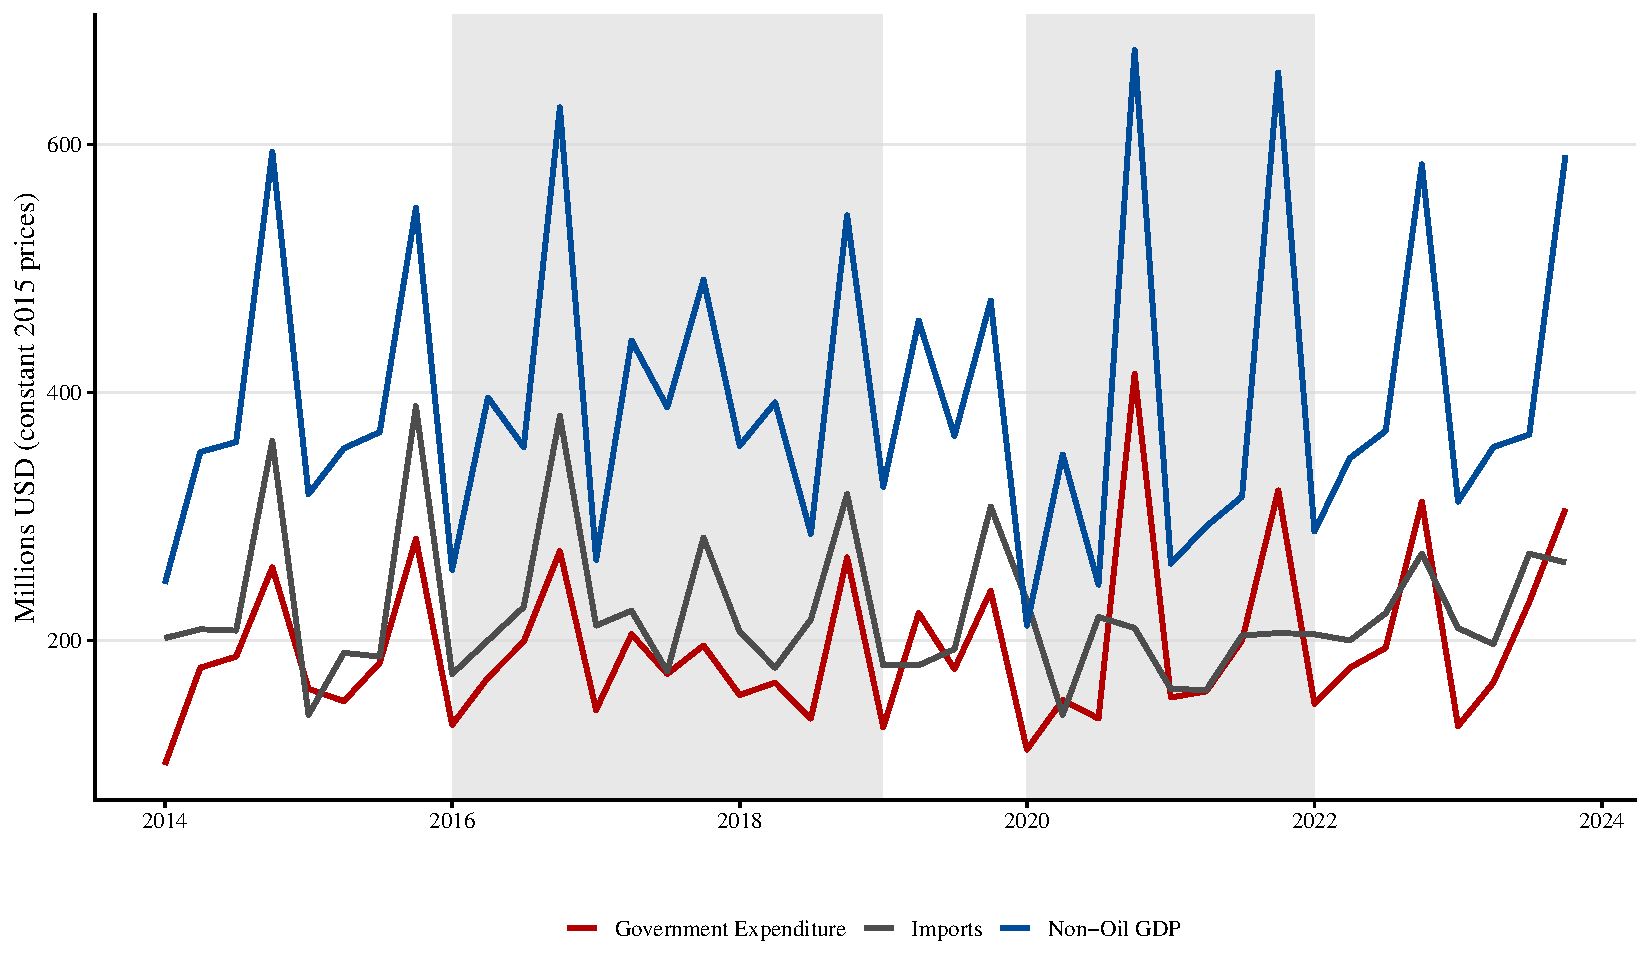
\includegraphics[width=\textwidth]{../graphics/figure_1_macro_levels_official.pdf}
  \caption{Levels}
\end{subfigure}\hfill
\begin{subfigure}[t]{0.49\textwidth}
  \centering
  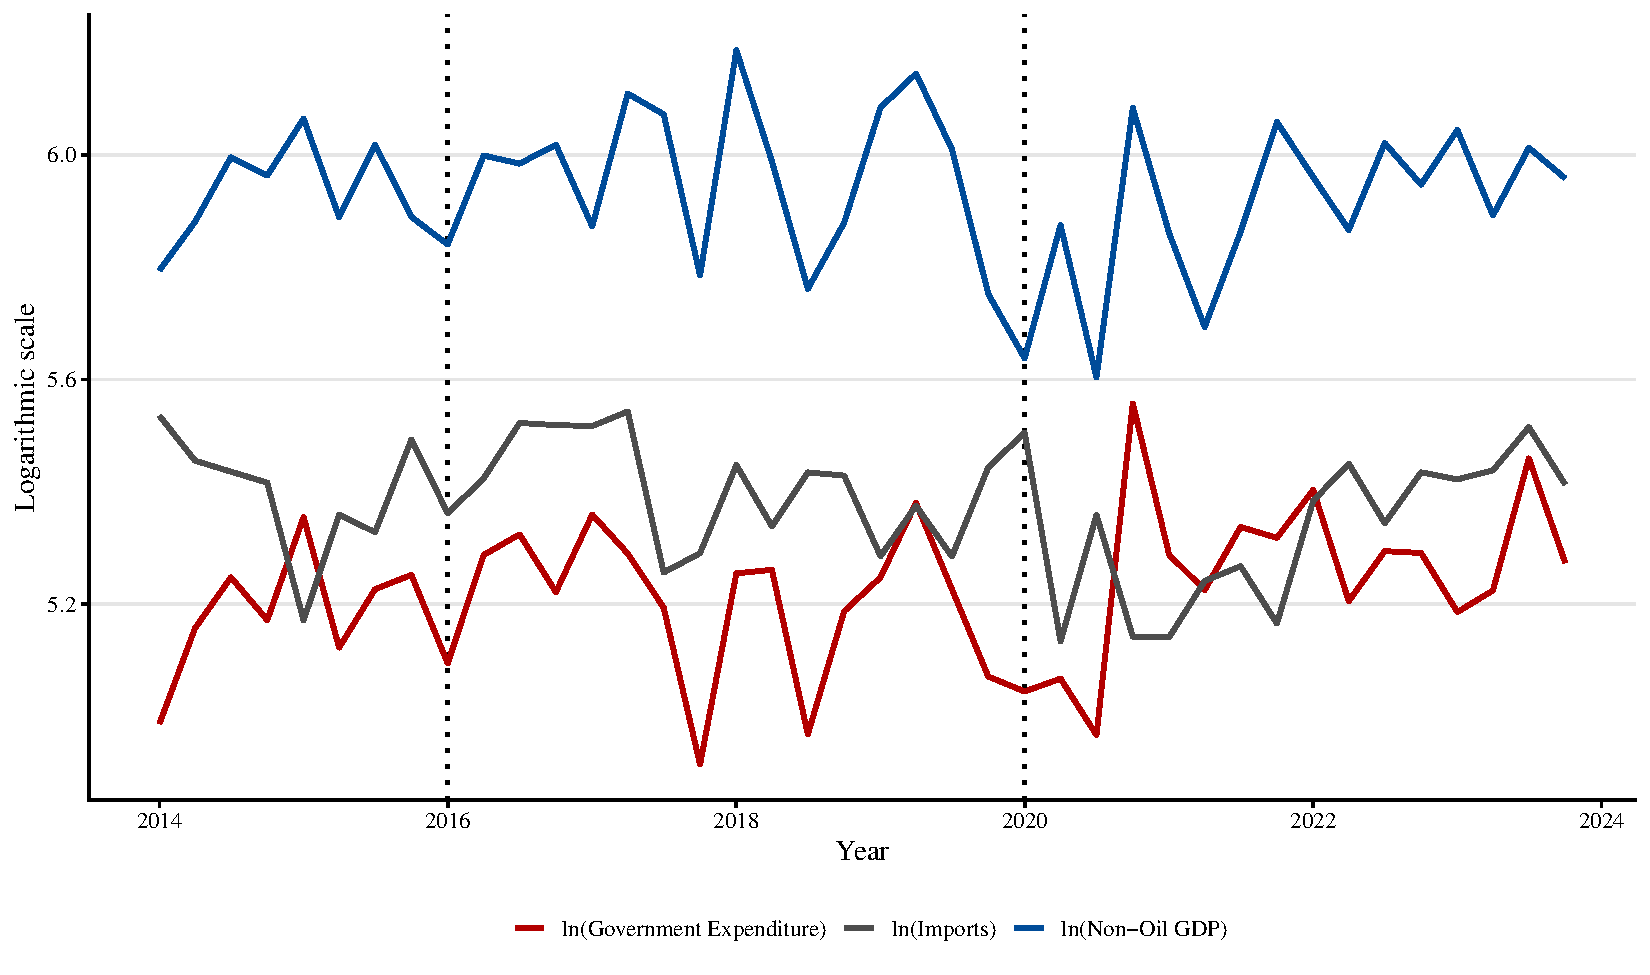
\includegraphics[width=\textwidth]{../graphics/figure_2_macro_log_official.pdf}
  \caption{Logarithms}
\end{subfigure}
\caption{Official quarterly macroeconomic series, 2014Q1--2023Q4. Gray areas mark the 2016--2018 and 2020--2021 event windows. Units: millions of USD at constant 2015 prices. Source: Author's elaboration from INETL, DNE, and BCTL data.}
\label{fig:macro}
\end{figure}

Figure~\ref{fig:macro_long} in~\ref{sec:appendix_long} shows the corresponding long-sample series. The contrast in high-frequency variation is visible: the interpolated series follow smooth trends, while the official series display substantial quarter-to-quarter variation.

\section{Empirical strategy}
\label{sec:method}

\subsection{Bayesian VAR}
\label{sec:bvar}

The baseline official model is a three-variable BVAR in logarithms:
\[
y_t = \left(\ln \text{gov}_t,\ \ln \text{imports}_t,\ \ln \text{GDP}_t\right)' ,
\]
with two lags, a constant, and the two event dummies. The variables are ordered with government expenditure first, so the fiscal shock is recursively identified: government expenditure does not respond contemporaneously to imports or GDP, while both can respond to the fiscal shock within the quarter. A second ordering places GDP first and government expenditure second, allowing expenditure to react to activity within the quarter. The comparison between orderings is a sensitivity check, not a test that eliminates all identification assumptions.

The prior is a Minnesota prior with hierarchical selection of the overall tightness $\lambda$. The prior mode of $\lambda$ is 0.2, with support $[0.001,3]$; $\alpha$ has mode 2 and support $[1,3]$; the scale $\psi$ is set to the square root of the variance of the first differences of each series, with the package's default bounds. The sampler uses 100,000 draws, 20,000 burn-in draws, and thinning every 20 draws, leaving 4,000 retained draws. Impulse responses are computed for 12 quarters with 68\% and 90\% credible intervals.

The three-variable specification is chosen because the official sample has only 40 observations. A five-variable model that adds the CPI and private credit has a maximum companion modulus above one (Table~\ref{tab:stability}); the additional dynamics are not supported by the data. The five-variable model is reported as a robustness check, not used for inference. The long sample, with 88 observations, supports both the three- and five-variable specifications.

\subsection{Local projections}
\label{sec:lp}

Local projections provide a complementary estimate that does not rely on the full VAR dynamics. We estimate a three-variable VAR with the same variables, lags, and dummies, extract the recursively identified government expenditure shock, and project each outcome on the shock and its pre-determined controls:
\[
y_{t+h} = \alpha_h + \beta_h \varepsilon_t + \Gamma_h X_{t-1} + u_{t+h},
\]
where $X_{t-1}$ contains a constant, two lags of the three core variables, and the event dummies. The coefficient $\beta_h$ is the response at horizon $h$. Standard errors are Newey--West HAC with bandwidth $\min(h+1,6)$. The shock is normalized so that the impact response of government expenditure is 1\%, which makes the LP coefficients directly comparable to the BVAR elasticities. We report horizons 0--12.

\subsection{Stability and stationarity}
\label{sec:stability}

Table~\ref{tab:stability} reports the maximum modulus of the companion matrix for each specification. The official three-variable model is stable (0.795), as are the long-sample three- and five-variable models (0.983 and 0.993). The official five-variable model is unstable (1.089), and we do not interpret its impulse responses. The hybrid model, which replaces the official government series with the broader interpolated ADB series while keeping official outcomes, is stable (0.940). The unadjusted official model is also stable (0.701).

\begin{table}[htbp]
\centering
\small
\caption{Companion-matrix stability}
\label{tab:stability}
\begin{tabular}{@{}llccc@{}}
\toprule
Model & Sample & Observations & Max.\ modulus & Stable \\
\midrule
3-variable BVAR & Official, 2014--2023 & 40 & 0.795 & Yes \\
5-variable BVAR & Official, 2014--2023 & 40 & 1.089 & No \\
3-variable BVAR, NSA & Official, 2014--2023 & 40 & 0.701 & Yes \\
3-variable BVAR & Long, 2002--2023 & 88 & 0.983 & Yes \\
5-variable BVAR & Long, 2002--2023 & 88 & 0.993 & Yes \\
3-variable BVAR & Hybrid, 2014--2023 & 40 & 0.940 & Yes \\
\bottomrule
\end{tabular}
\par\vspace{0.3em}
\begin{minipage}{0.95\textwidth}
\footnotesize\textit{Note:} Maximum modulus of the eigenvalues of the companion matrix at the posterior mean. A value below one indicates a stable VAR. Source: Author's elaboration.
\end{minipage}
\end{table}

Unit-root tests are reported in Table~\ref{tab:stationarity}. We apply augmented Dickey--Fuller \parencite{dickeyfuller1979}, KPSS \parencite{kpss1992}, and Zivot--Andrews \parencite{zivot1992} tests. The evidence is mixed: ADF tests do not reject a unit root for most series at the 5\% level, while KPSS tests reject stationarity for the CPI and credit. The Zivot--Andrews test rejects the unit root for non-oil GDP with a break in 2019Q4, but not for the other series. Given the short sample and the mixed evidence, we estimate the BVAR in levels with a Minnesota prior, which shrinks toward a random-walk representation and is robust to persistent series. The long-sample tests are reported in~\ref{sec:appendix_long}.

\begin{table}[htbp]
\centering
\small
\caption{Unit-root and stationarity tests, official sample}
\label{tab:stationarity}
\begin{tabular}{@{}lcccccl@{}}
\toprule
Series & ADF ($p$) & KPSS ($p$) & ZA ($t$) & 5\% CV & Break & Stationary? \\
\midrule
\texttt{ln\_gov\_exp} & 0.093 & 0.100 & $-4.66$ & $-5.08$ & 2020Q3 & No \\
\texttt{ln\_gdp\_non} & 0.259 & 0.100 & $-6.24$ & $-5.08$ & 2019Q4 & Yes \\
\texttt{ln\_imports} & 0.360 & 0.100 & $-3.85$ & $-5.08$ & 2020Q1 & No \\
\texttt{ln\_cpi} & 0.976 & 0.010 & $-2.76$ & $-5.08$ & 2019Q4 & No \\
\texttt{ln\_credit} & 0.764 & 0.010 & $-3.77$ & $-5.08$ & 2021Q1 & No \\
\bottomrule
\end{tabular}
\par\vspace{0.3em}
\begin{minipage}{0.95\textwidth}
\footnotesize\textit{Note:} ADF: $H_0$ unit root. KPSS: $H_0$ stationarity. ZA: $H_0$ unit root with a structural break (model ``both'', two lags); a $t$-statistic below the critical value rejects $H_0$. Source: Author's elaboration.
\end{minipage}
\end{table}

\section{Results}
\label{sec:results}

\subsection{Official BVAR}
\label{sec:official_bvar}

Figure~\ref{fig:irf_official} shows the impulse responses to a one-unit structural government expenditure innovation under the two orderings. The responses are rescaled to a 1\% increase in government expenditure in Table~\ref{tab:bvar_elasticities}; the figures preserve the original shock scale. The fiscal shock is persistent but transitory: government expenditure itself rises and then returns toward zero. Imports do not display the large positive response found in the long sample. Under order 1, the median import response is $-0.03\%$ at impact, $0.09\%$ after three quarters, and essentially zero thereafter; the 68\% interval includes zero at all horizons. The GDP response is positive at impact ($0.52\%$) but reverses by the third quarter ($-0.09\%$) and is not distinguishable from zero at longer horizons.

\begin{figure}[htbp]
\centering
\begin{subfigure}[t]{0.49\textwidth}
  \centering
  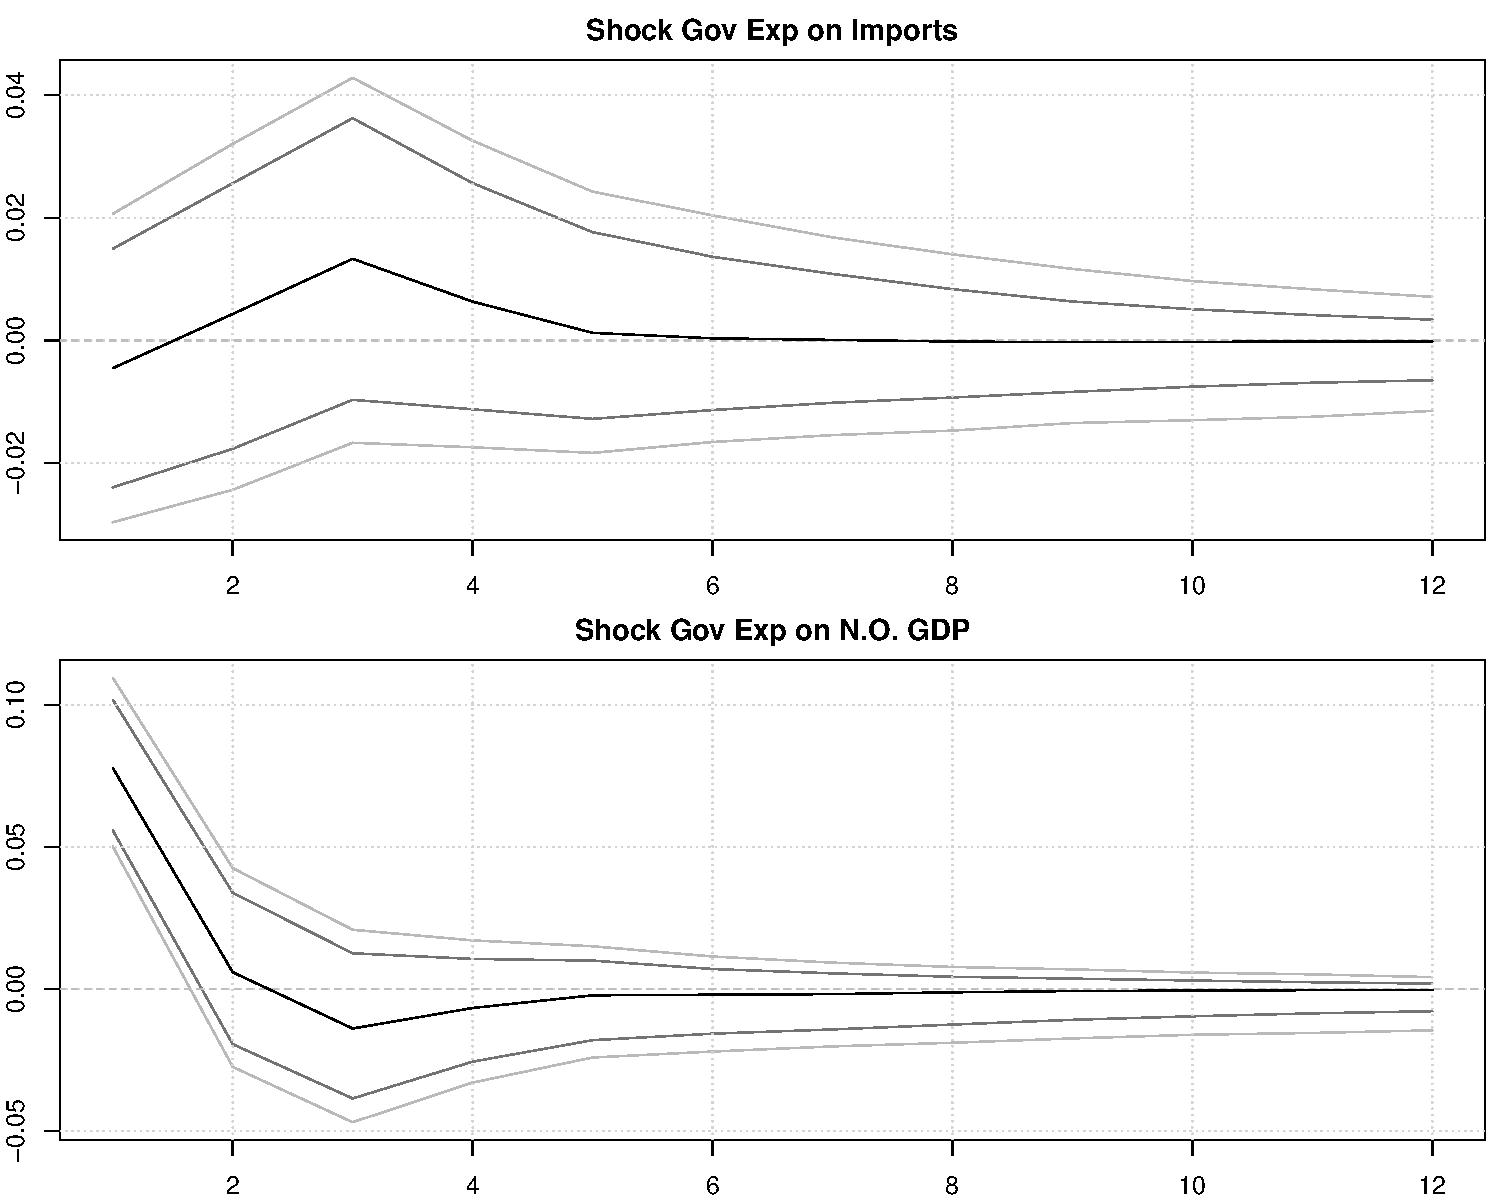
\includegraphics[width=\textwidth]{../graphics/irf_gov_shock_order_1_official_3var.pdf}
  \caption{Order 1}
\end{subfigure}\hfill
\begin{subfigure}[t]{0.49\textwidth}
  \centering
  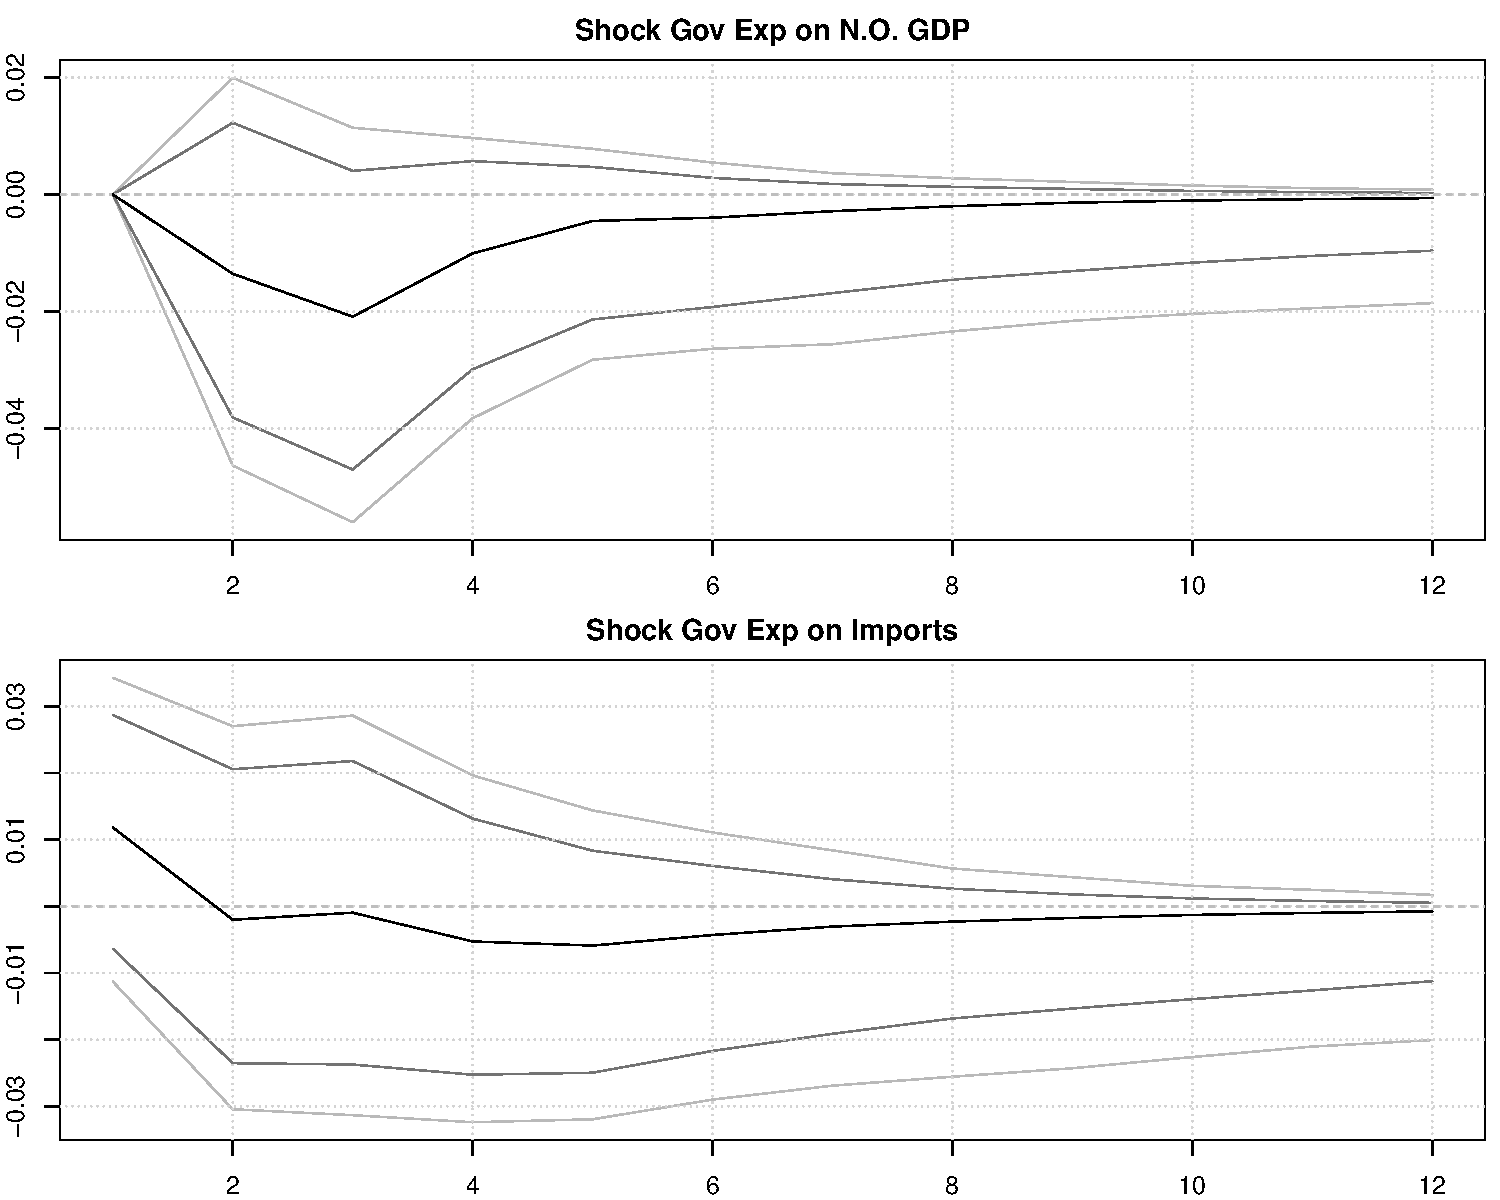
\includegraphics[width=\textwidth]{../graphics/irf_gov_shock_order_2_official_3var.pdf}
  \caption{Order 2}
\end{subfigure}
\caption{Official-sample BVAR impulse responses to a government expenditure shock, orders 1 and 2. Bands: 68\% and 90\%. Units: response to a one-unit structural innovation. Table~\ref{tab:bvar_elasticities} reports the responses rescaled to a 1\% increase in government expenditure. Source: Author's elaboration.}
\label{fig:irf_official}
\end{figure}

\begin{table}[htbp]
\centering
\small
\caption{BVAR responses to a 1\% government expenditure shock (percent)}
\label{tab:bvar_elasticities}
\resizebox{\textwidth}{!}{%
\begin{tabular}{@{}llccc@{}}
\toprule
 & & Official 3-variable & Long 3-variable & Long 5-variable \\
Response & Horizon & (2014--2023) & (2002--2023) & (2002--2023) \\
\midrule
Imports & 1 & $-0.03\ [-0.16,\ 0.10]$ & $0.34\ [0.21,\ 0.48]$ & $0.35\ [0.22,\ 0.49]$ \\
Imports & 2 & $0.03\ [-0.12,\ 0.17]$ & $0.78\ [0.55,\ 1.02]$ & $0.81\ [0.59,\ 1.05]$ \\
Imports & 3 & $0.09\ [-0.06,\ 0.24]$ & $1.22\ [0.87,\ 1.57]$ & $1.25\ [0.92,\ 1.58]$ \\
Imports & 6 & $0.00\ [-0.08,\ 0.09]$ & $2.08\ [1.48,\ 2.73]$ & $2.00\ [1.45,\ 2.62]$ \\
Imports & 7 & $0.00\ [-0.07,\ 0.07]$ & $2.15\ [1.49,\ 2.91]$ & $2.05\ [1.44,\ 2.75]$ \\
Imports & 12 & $0.00\ [-0.04,\ 0.02]$ & $1.30\ [0.50,\ 2.33]$ & $1.26\ [0.41,\ 2.31]$ \\
Non-oil GDP & 1 & $0.52\ [0.37,\ 0.68]$ & $-0.01\ [-0.06,\ 0.04]$ & $-0.01\ [-0.06,\ 0.04]$ \\
Non-oil GDP & 2 & $0.04\ [-0.13,\ 0.23]$ & $0.02\ [-0.07,\ 0.11]$ & $0.00\ [-0.08,\ 0.07]$ \\
Non-oil GDP & 3 & $-0.09\ [-0.26,\ 0.08]$ & $0.08\ [-0.05,\ 0.20]$ & $0.04\ [-0.06,\ 0.14]$ \\
Non-oil GDP & 6 & $-0.01\ [-0.10,\ 0.05]$ & $0.31\ [0.09,\ 0.53]$ & $0.29\ [0.15,\ 0.44]$ \\
Non-oil GDP & 7 & $-0.01\ [-0.09,\ 0.04]$ & $0.38\ [0.13,\ 0.64]$ & $0.37\ [0.22,\ 0.54]$ \\
Non-oil GDP & 12 & $0.00\ [-0.05,\ 0.01]$ & $0.52\ [0.17,\ 0.92]$ & $0.59\ [0.36,\ 0.86]$ \\
\bottomrule
\end{tabular}}
\par\vspace{0.3em}
\begin{minipage}{0.95\textwidth}
\footnotesize\textit{Note:} Posterior medians with 68\% credible intervals in brackets. Responses are rescaled so that the impact response of government expenditure is 1\%. A value of 0.34 means that a 1\% increase in government expenditure is associated with a 0.34\% increase in imports. The long 5-variable model is the specification used in earlier versions of the paper. Source: Author's elaboration.
\end{minipage}
\end{table}

The five-variable official BVAR produces qualitatively similar results but is unstable. Its import response is small and the GDP response is short-lived. Because the maximum companion modulus is 1.089, we do not use it for inference. The instability is a symptom of the short sample: with 40 observations and two lags, the five-variable system has more parameters than the data can support. This is not a defect of the estimator; it is a constraint of the available official data.

\subsection{Official local projections}
\label{sec:official_lp}

Figure~\ref{fig:lp_official} and Table~\ref{tab:lp_elasticities} report the local-projection estimates. The official import response is small and imprecisely estimated: $-0.12\%$ at impact, $0.10\%$ after one quarter, $-0.38\%$ after two quarters, and $0.34$--$0.36\%$ after six to twelve quarters. The negative response at two quarters is statistically distinguishable from zero at the 68\% level, but its magnitude is negligible. The positive responses at six and twelve quarters are also small, below 0.4\%. Non-oil GDP is close to zero at all horizons, with a negative point estimate at three quarters ($-0.23\%$) and a positive but insignificant estimate at twelve quarters ($0.37\%$). The CPI and credit responses are close to zero.

\begin{figure}[htbp]
\centering
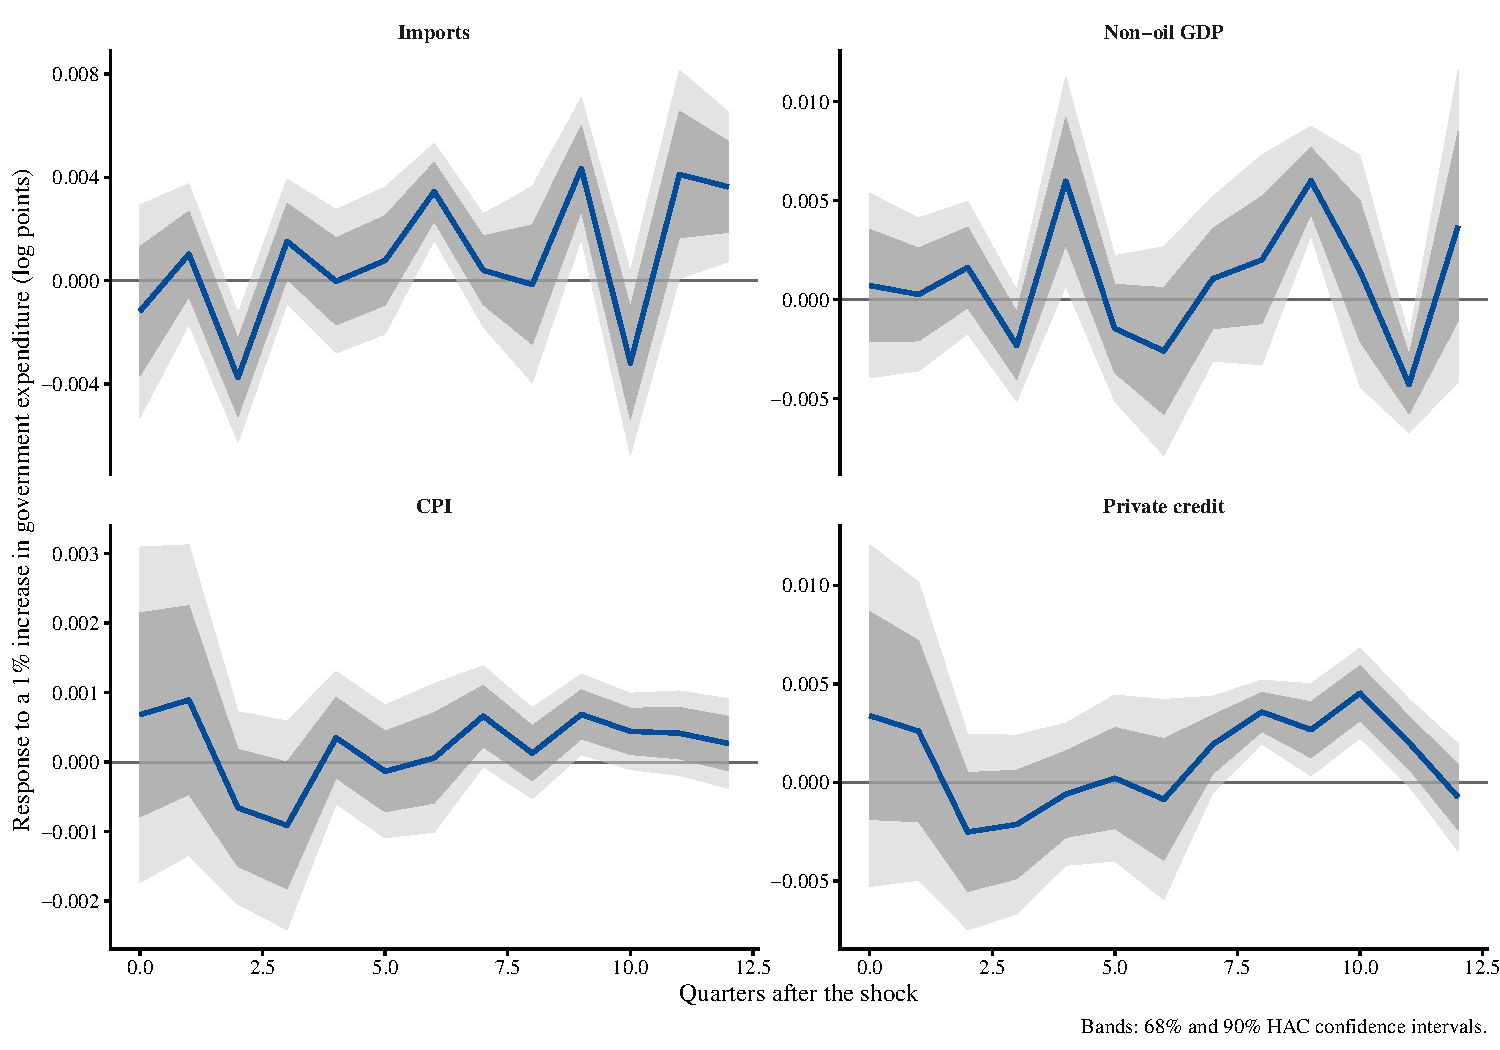
\includegraphics[width=0.95\textwidth]{../graphics/lp_irf_official.pdf}
\caption{Official-sample local projections to a 1\% government expenditure shock. Bands: 68\% and 90\% Newey--West HAC confidence intervals. Source: Author's elaboration.}
\label{fig:lp_official}
\end{figure}

\begin{table}[htbp]
\centering
\small
\caption{Local-projection responses to a 1\% government expenditure shock (percent)}
\label{tab:lp_elasticities}
\begin{tabular}{@{}lccc@{}}
\toprule
Response & Horizon & Official sample & Long sample \\
\midrule
Imports & 0 & $-0.12\ [-0.37,\ 0.13]$ & $8.11\ [7.43,\ 8.79]$ \\
Imports & 1 & $0.10\ [-0.06,\ 0.27]$ & $17.54\ [15.73,\ 19.35]$ \\
Imports & 2 & $-0.38\ [-0.53,\ -0.22]$ & $23.62\ [20.66,\ 26.58]$ \\
Imports & 3 & $0.15\ [0.01,\ 0.30]$ & $23.65\ [19.10,\ 28.21]$ \\
Imports & 6 & $0.34\ [0.23,\ 0.46]$ & $0.71\ [-7.52,\ 8.94]$ \\
Imports & 12 & $0.36\ [0.19,\ 0.54]$ & $11.05\ [3.97,\ 18.14]$ \\
Non-oil GDP & 0 & $0.07\ [-0.21,\ 0.36]$ & $0.15\ [-0.14,\ 0.44]$ \\
Non-oil GDP & 1 & $0.03\ [-0.21,\ 0.26]$ & $0.57\ [-0.15,\ 1.29]$ \\
Non-oil GDP & 2 & $0.16\ [-0.04,\ 0.37]$ & $1.14\ [0.03,\ 2.25]$ \\
Non-oil GDP & 3 & $-0.23\ [-0.40,\ -0.06]$ & $1.74\ [0.37,\ 3.11]$ \\
Non-oil GDP & 6 & $-0.26\ [-0.58,\ 0.06]$ & $2.90\ [0.81,\ 5.00]$ \\
Non-oil GDP & 12 & $0.37\ [-0.11,\ 0.85]$ & $6.25\ [4.26,\ 8.24]$ \\
\bottomrule
\end{tabular}
\par\vspace{0.3em}
\begin{minipage}{0.95\textwidth}
\footnotesize\textit{Note:} Point estimates with 68\% Newey--West HAC confidence intervals in brackets. The shock is normalized so that the impact response of government expenditure is 1\%. Source: Author's elaboration.
\end{minipage}
\end{table}

Taken together, the official BVAR and LP provide no evidence of a large or persistent import leakage. The BVAR estimates an import response below 0.1\% at short horizons; the LP estimates a small positive response of about 0.3--0.4\% at longer horizons, but it is an order of magnitude smaller than the long-sample estimates and does not support the view that fiscal stimulus is largely spent abroad. The GDP response is fragile: the BVAR finds a short-lived positive impact effect, while the LP finds a small negative effect at three quarters. The robust conclusion is that the official data do not identify a positive output effect that persists.

\subsection{The long-sample result}
\label{sec:long_results}

For comparison, Figure~\ref{fig:irf_long} and the last two columns of Table~\ref{tab:bvar_elasticities} report the long-sample BVAR. The same three-variable specification is stable and estimates a significant import response: 0.34\% at impact, 1.22\% after three quarters, 2.08\% after six quarters, and 2.15\% at the peak after seven quarters. The 68\% interval excludes zero at every horizon shown. Non-oil GDP responds with a lag and remains modest: 0.31\% after six quarters and 0.52\% after twelve. The five-variable long-sample model, which is the specification used in earlier work, gives nearly identical results (0.35\% at impact, 2.05\% at the peak).

\begin{figure}[htbp]
\centering
\begin{subfigure}[t]{0.49\textwidth}
  \centering
  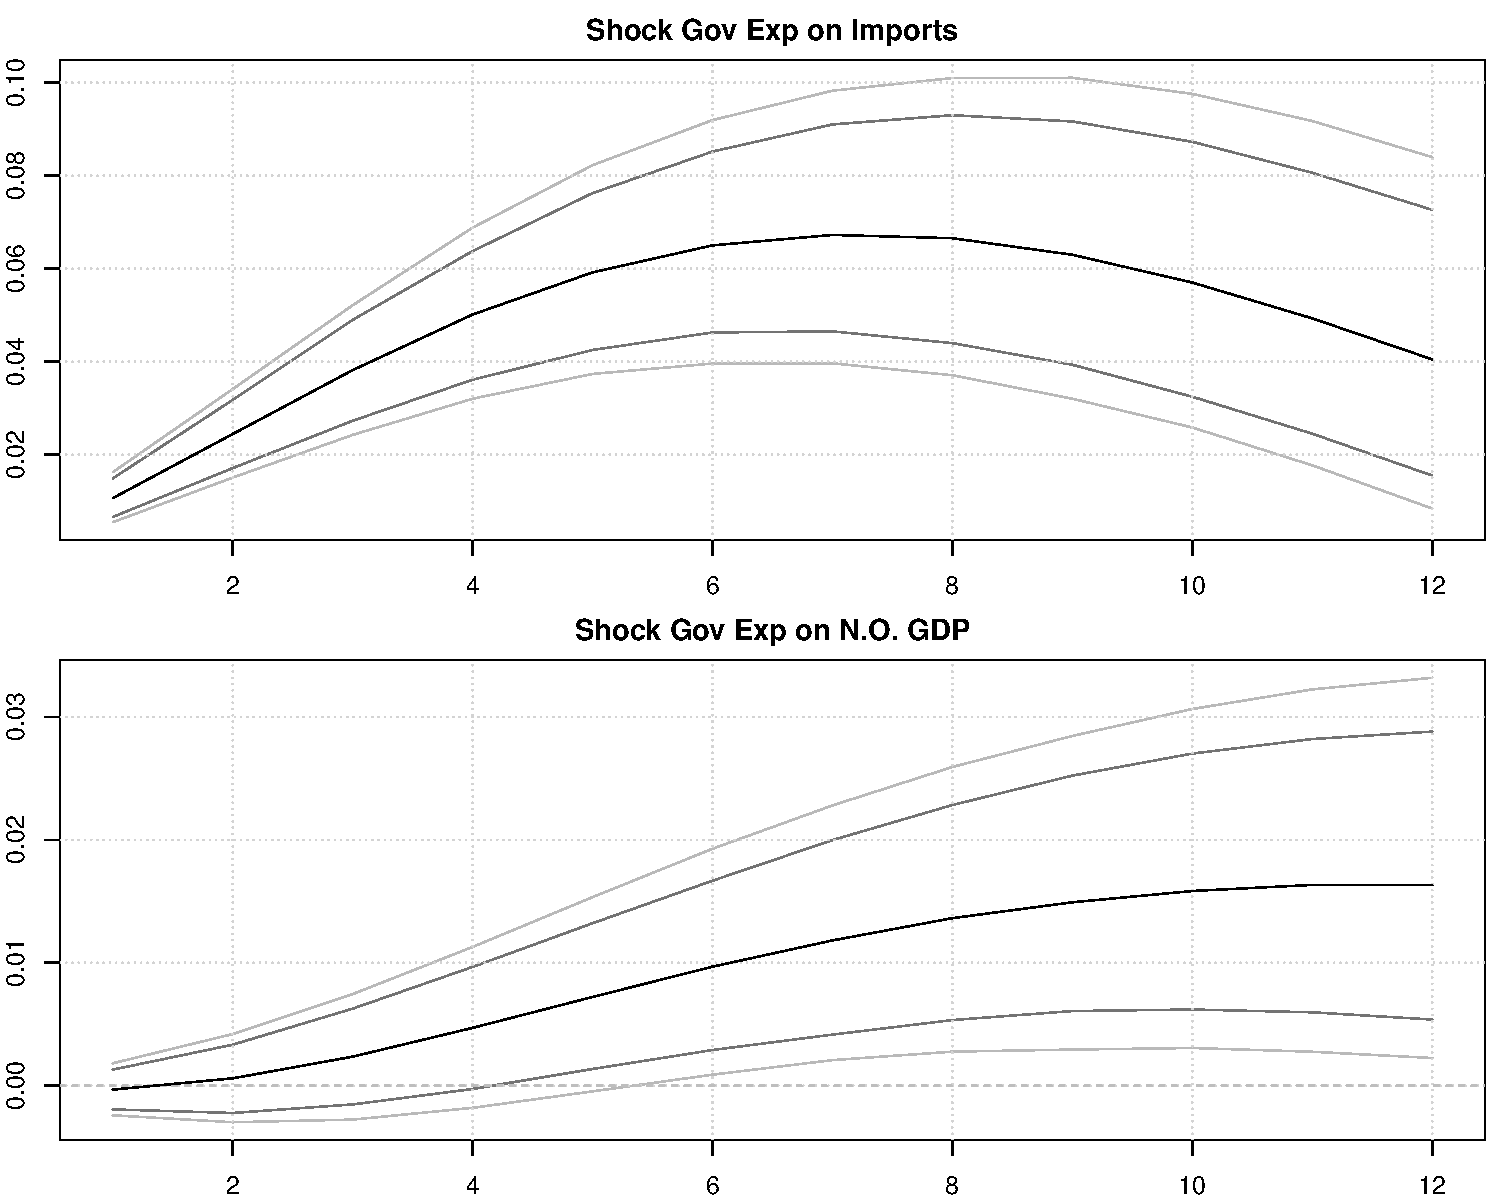
\includegraphics[width=\textwidth]{../graphics/irf_gov_shock_order_1_long_3var.pdf}
  \caption{Order 1}
\end{subfigure}\hfill
\begin{subfigure}[t]{0.49\textwidth}
  \centering
  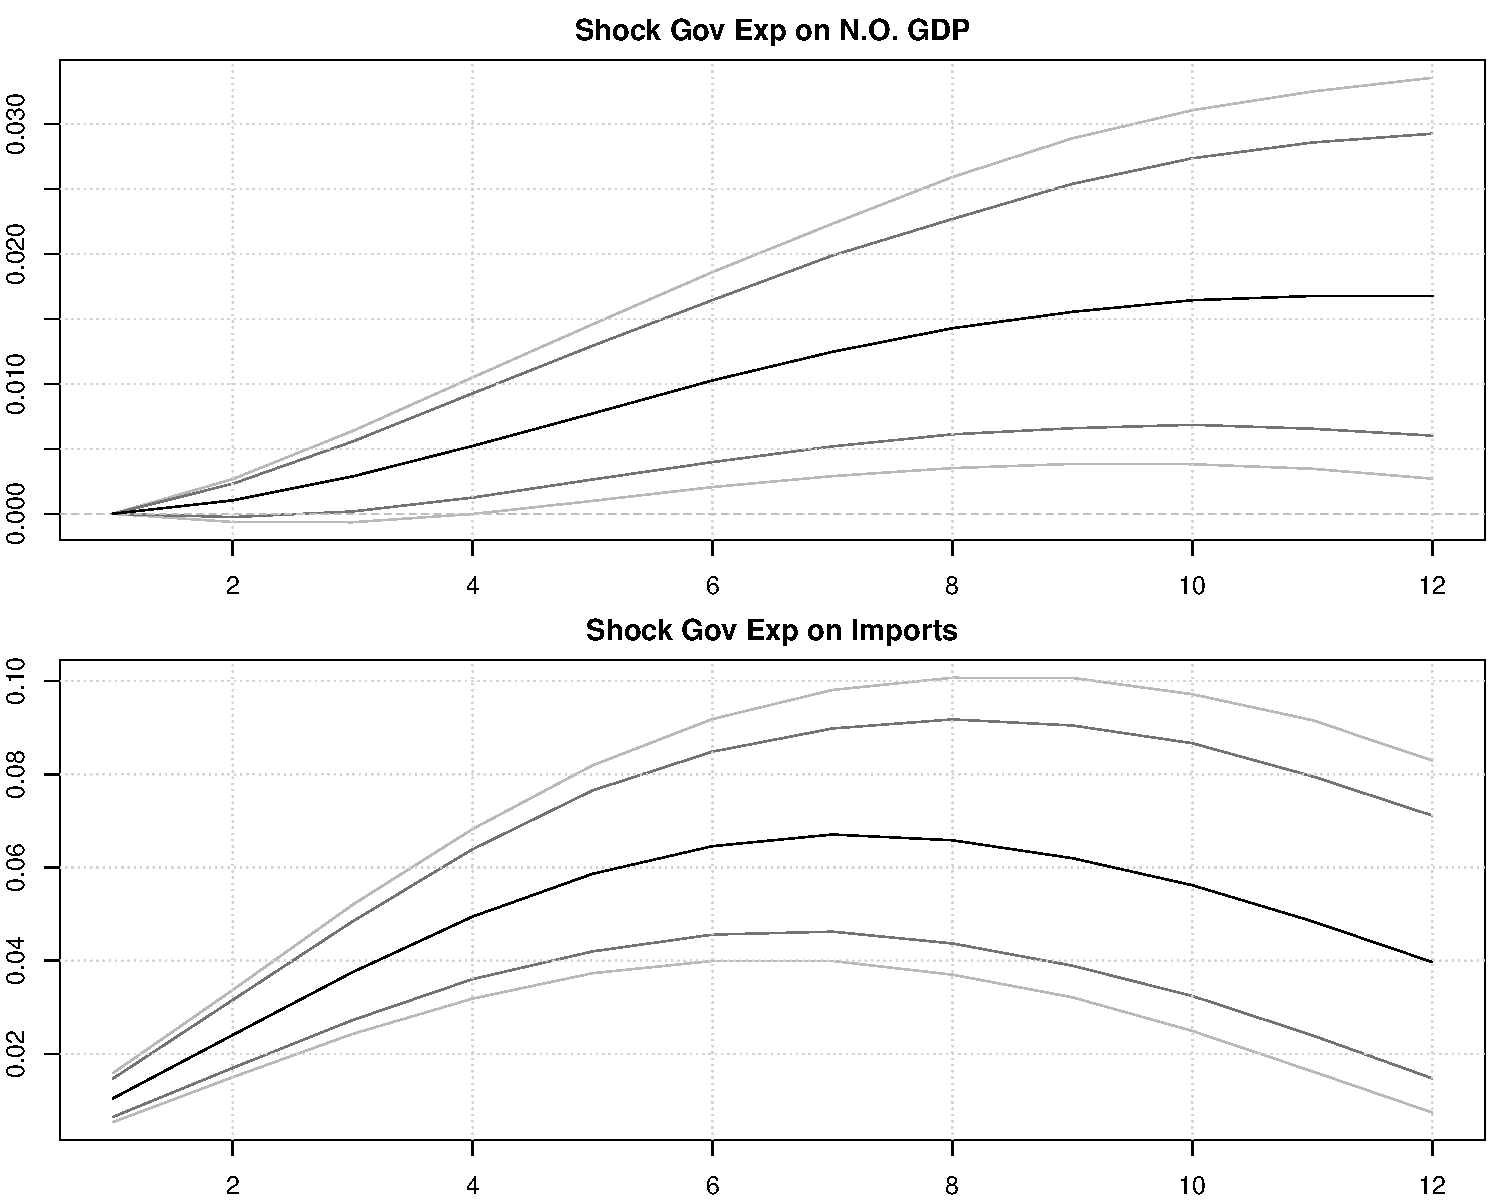
\includegraphics[width=\textwidth]{../graphics/irf_gov_shock_order_2_long_3var.pdf}
  \caption{Order 2}
\end{subfigure}
\caption{Long-sample BVAR impulse responses to a government expenditure shock, orders 1 and 2. Bands: 68\% and 90\%. Units: response to a one-unit structural innovation. Table~\ref{tab:bvar_elasticities} reports the responses rescaled to a 1\% increase in government expenditure. Source: Author's elaboration.}
\label{fig:irf_long}
\end{figure}

The long-sample LP estimates are larger still (Figure~\ref{fig:lp_long} and Table~\ref{tab:lp_elasticities}). The import response rises from 8.1\% at impact to 23.6\% after two quarters and 23.7\% after three quarters, then becomes imprecise at intermediate horizons. The GDP response rises gradually to 6.25\% after twelve quarters. The LP and BVAR agree on the qualitative pattern: in the long sample, imports respond earlier and more strongly than GDP. The magnitude differs because the LP imposes less structure and estimates the response separately at each horizon; the LP estimates are larger at the peak but less stable across horizons, and they should be read as complementary evidence rather than a strict upper bound.

\begin{figure}[htbp]
\centering
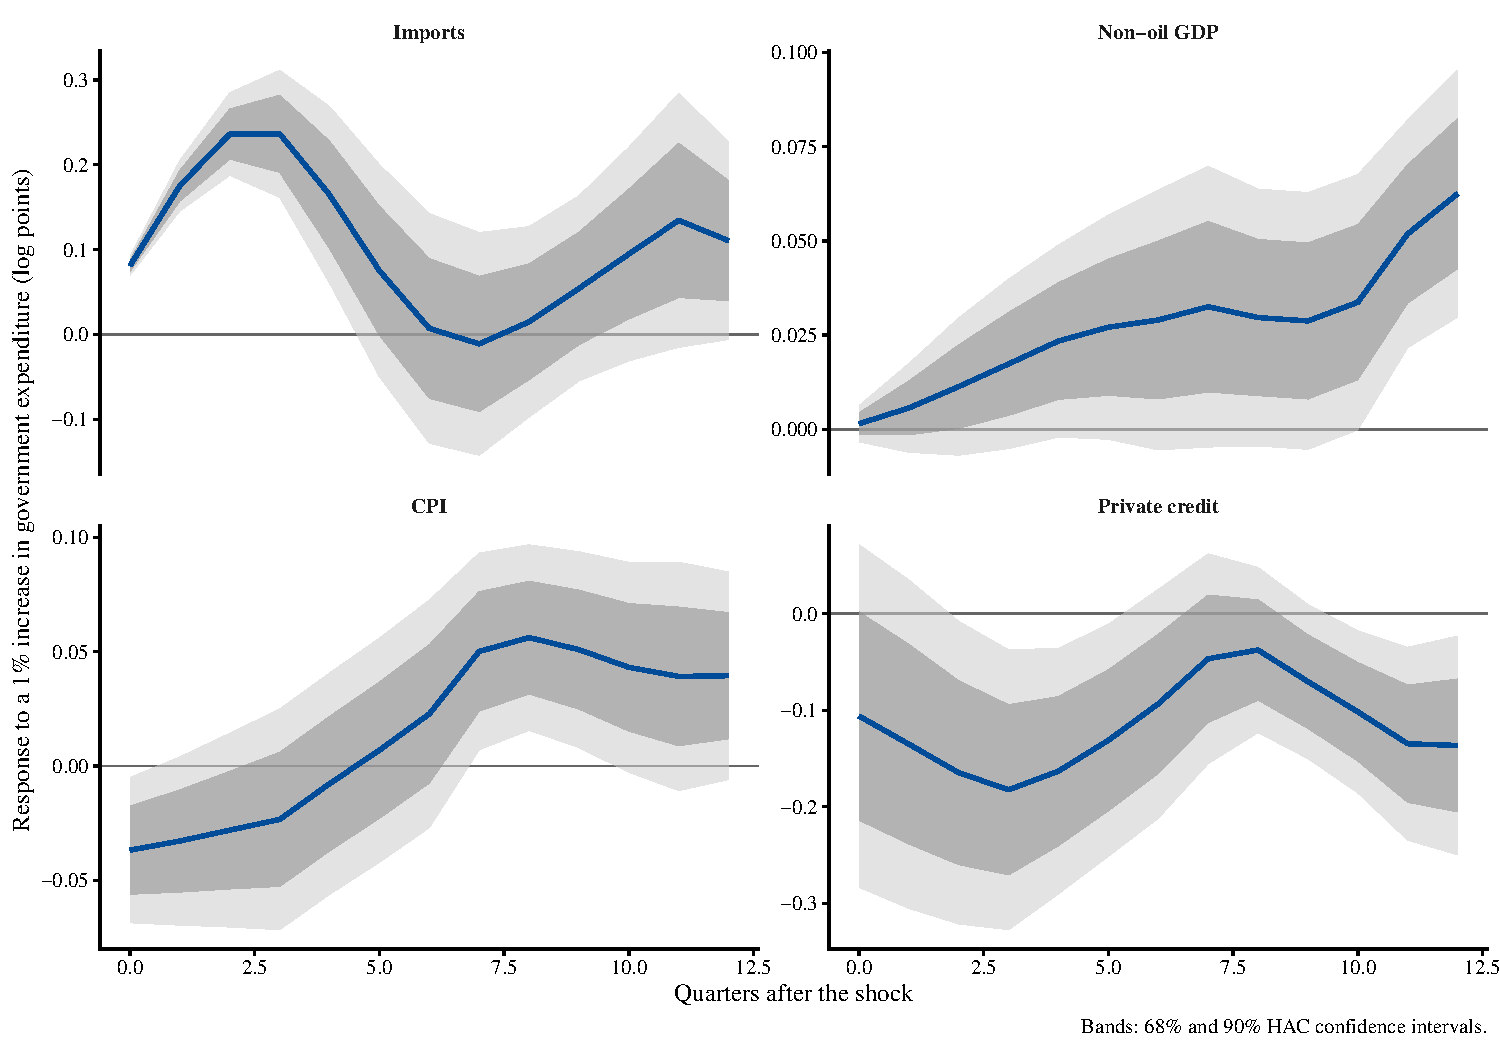
\includegraphics[width=0.95\textwidth]{../graphics/lp_irf_long.pdf}
\caption{Long-sample local projections to a 1\% government expenditure shock. Bands: 68\% and 90\% Newey--West HAC confidence intervals. Source: Author's elaboration.}
\label{fig:lp_long}
\end{figure}

\subsection{Why the two samples disagree}
\label{sec:artifact}

The contrast between the official and long-sample results is not driven by the estimator, the prior, or the identification. The same three-variable BVAR, with the same lags, prior, and ordering, produces a near-zero import response in the official sample and a large, significant response in the long sample. The difference must therefore come from the data: either their construction or the sample period.

The mechanism is temporal disaggregation. Denton--Cholette distributes each annual total across quarters using a smoothness criterion. When all series are disaggregated in this way, they share a common annual benchmark and a common smooth trend. The resulting quarterly series have little high-frequency independent variation (Table~\ref{tab:volatility}). A VAR estimated on these series sees a strong positive comovement between government expenditure and imports, and the recursive identification attributes it to the fiscal shock. The long-sample impulse response is large because the interpolated series move together by construction.

The official data break this comovement. Quarterly government expenditure, GDP, and imports each contain independent high-frequency variation. The fiscal shock is therefore identified from a much smaller and noisier component of the data, and the estimated import response is small. The official BVAR's maximum companion modulus is below one, so the result is not a symptom of instability.

Two additional checks support this interpretation. First, the hybrid model replaces the official government series with the broader ADB government series, interpolated to quarterly frequency, while keeping official GDP and imports. If the absence of leakage were due to the narrow official measure of government consumption, the hybrid should restore the leakage. It does not: the hybrid is stable (0.940) and its import response is between $-0.3\%$ and $0.2\%$ at all horizons. Second, the unadjusted official model, which uses quarterly dummies instead of X-13 adjustment, produces a short-lived first-quarter import spike (0.39\%) but no persistent response; the seasonal spike disappears by the second quarter. Neither check restores the long-sample result. The leakage is a property of the jointly interpolated data, not of the fiscal measure alone. One caveat is that the long sample also covers 2002--2013, a period for which official quarterly outcomes are unavailable. The hybrid check holds the sample period and the outcome series fixed and varies only the fiscal measure; because it does not restore the leakage, the result is unlikely to be driven by the broader fiscal measure alone. The joint interpolation of the outcome series remains the most plausible mechanism, but the comparison cannot fully separate interpolation from period-specific shocks.

The five-variable official model is unstable, but its point responses are also small and short-lived. We do not interpret them because the companion roots exceed one. The instability is consistent with the short sample: adding the CPI and credit doubles the number of parameters without adding enough observations. The long sample supports the five-variable model, which is why earlier work could estimate it; the cost is that the additional observations are interpolated.

\subsection{Robustness}
\label{sec:robustness}

Table~\ref{tab:robustness} collects the alternative specifications. The official unadjusted model is stable and produces a first-quarter import response of 0.39\%, but the response turns negative in the second and third quarters and is essentially zero thereafter. The official five-variable model is unstable and is not used for inference. The hybrid model is stable and produces import responses between $-0.3\%$ and $0.2\%$, with intervals that include zero. The long three- and five-variable models are stable and produce significant import responses of about 2\% at the peak. The qualitative conclusion is unchanged across specifications: the official data do not support a large, persistent leakage; the long interpolated data do.

\begin{table}[htbp]
\centering
\small
\caption{Robustness: stability and selected responses}
\label{tab:robustness}
\resizebox{\textwidth}{!}{%
\begin{tabular}{@{}lcccccc@{}}
\toprule
Model & Sample & Max.\ modulus & Imports $h=1$ & Imports $h=3$ & Imports $h=12$ & GDP $h=3$ \\
\midrule
Official 3-var & 2014--2023 & 0.795 & $-0.03$ & $0.09$ & $0.00$ & $-0.09$ \\
Official 5-var & 2014--2023 & 1.089 & $-0.06$ & $0.05$ & $0.00$ & $-0.05$ \\
Official 3-var, NSA & 2014--2023 & 0.701 & $0.39$ & $-0.09$ & $0.00$ & $0.04$ \\
Long 3-var & 2002--2023 & 0.983 & $0.34$ & $1.22$ & $1.30$ & $0.08$ \\
Long 5-var & 2002--2023 & 0.993 & $0.35$ & $1.25$ & $1.26$ & $0.04$ \\
Hybrid 3-var & 2014--2023 & 0.940 & $-0.28$ & $-0.03$ & $0.16$ & $-0.19$ \\
\bottomrule
\end{tabular}}
\par\vspace{0.3em}
\begin{minipage}{0.95\textwidth}
\footnotesize\textit{Note:} Responses are medians in percent, rescaled to a 1\% increase in government expenditure. The hybrid model uses the interpolated ADB government series with official GDP and imports. The official 5-variable model is unstable and its responses are reported only for completeness. Source: Author's elaboration.
\end{minipage}
\end{table}

The FEVD tells the same story. In the official three-variable model, the fiscal shock explains 1.2\% of import variance at the one-quarter horizon, 6.2\% after six quarters, and 6.8\% after twelve quarters; for GDP, the shares are 27.5\%, 24.5\%, and 24.1\%. In the long three-variable model, the fiscal shock explains 7.3\% of import variance at one quarter, 34.5\% after six quarters, and 50.3\% after twelve quarters; for GDP, the shares are 0.6\%, 4.6\%, and 14.9\%. The long-sample fiscal shock is a dominant source of import fluctuations; the official fiscal shock is not. Figure~\ref{fig:fevd} presents the FEVDs.

\section{Conclusion}
\label{sec:conclusion}

This paper revisited the evidence on fiscal leakage in Timor-Leste using official quarterly national accounts. The main conclusion is that the strong leakage result obtained from interpolated data is not robust. With official data for 2014Q1--2023Q4, a stable three-variable BVAR and local projections estimate a small, imprecise import response, below 0.4\% at all horizons, and no persistent output effect. The long 2002--2023 sample built by Denton--Cholette disaggregation produces a large and significant import response, peaking near 2\% in the BVAR and 24\% in local projections. The difference is due to how the data are constructed, not the estimator or the identification.

The methodological lesson is that temporal disaggregation can generate spurious fiscal transmission. Because the interpolated series share a common annual benchmark and a common smooth trend, they comove mechanically. A VAR estimated on these series can attribute that comovement to a fiscal shock, producing a large and apparently precise leakage effect. The official data, which contain independent quarterly variation, do not support that interpretation. The hybrid experiment, which uses a smooth government series with official outcomes, is consistent with the interpretation that the artifact requires the joint interpolation of the outcome series, not just a smooth fiscal measure.

These findings have implications for policy analysis in data-limited economies. Estimates of fiscal multipliers and leakage based on interpolated quarterly data should be treated with caution, and they should be tested against official high-frequency data whenever available. For Timor-Leste, the official data do not provide evidence of a large import leakage, but they also do not provide a precise estimate of the fiscal multiplier. The small official-data responses are consistent with the existing estimates of 0.08--0.17 for the multiplier \parencite{worldbank2021,imf2024}. The short sample, the volatility of government expenditure, and the source differences between national-accounts and administrative data all limit precision. The appropriate conclusion is not that leakage is absent, but that the available official data do not support the large and persistent leakage estimated from interpolated series.

Further work should extend the official sample as new quarterly observations become available, explore alternative fiscal shocks based on budget execution data, and investigate whether the interpolation artifact is present in other small open economies.

\section*{Data and code availability}
\label{sec:repro}

We welcome readers to use, replicate, review, and extend this work. All code, processed data, and generated results are available in the public repository \url{https://github.com/Emerson-nic/Timor-Leste-fiscal-bvar}. The \texttt{README} documents the project structure, data sources, script execution order, and document compilation with LuaLaTeX and Biber. The official data are built by \texttt{scripts/00\_build\_quarterly\_official.R}; the BVAR is estimated by \texttt{scripts/07\_irf\_fevd.R} with \texttt{SAMPLE=official\_3var} or \texttt{SAMPLE=long\_3var}; the local projections are estimated by \texttt{scripts/08\_local\_projections.R}; and the hybrid robustness check is in \texttt{scripts/09\_hybrid\_robustness.R}. The dashboard data are prepared by \texttt{scripts/build\_dashboard\_data.R}, and the interactive dashboard is available at \url{https://connect.posit.cloud/em3r/content/01a068c1-99da-638d-1ba0-1254293e5a61}.

\printbibliography[title={References}]

\appendix
\renewcommand{\thesection}{Appendix \Alph{section}}

\section{Long-sample descriptive evidence}
\label{sec:appendix_long}

Figure~\ref{fig:macro_long} shows the long-sample series in levels and logs. The series are smooth by construction. The dotted lines in panel (b) mark the main breaks selected by BIC across the five series using the Bai--Perron procedure \parencite{baiperron1998,baiperron2003}. Table~\ref{tab:stationarity_long} reports the unit-root tests for the long sample. The evidence is again mixed, and the BVAR is estimated in levels with a Minnesota prior.

\begin{figure}[htbp]
\centering
\begin{subfigure}[t]{0.49\textwidth}
  \centering
  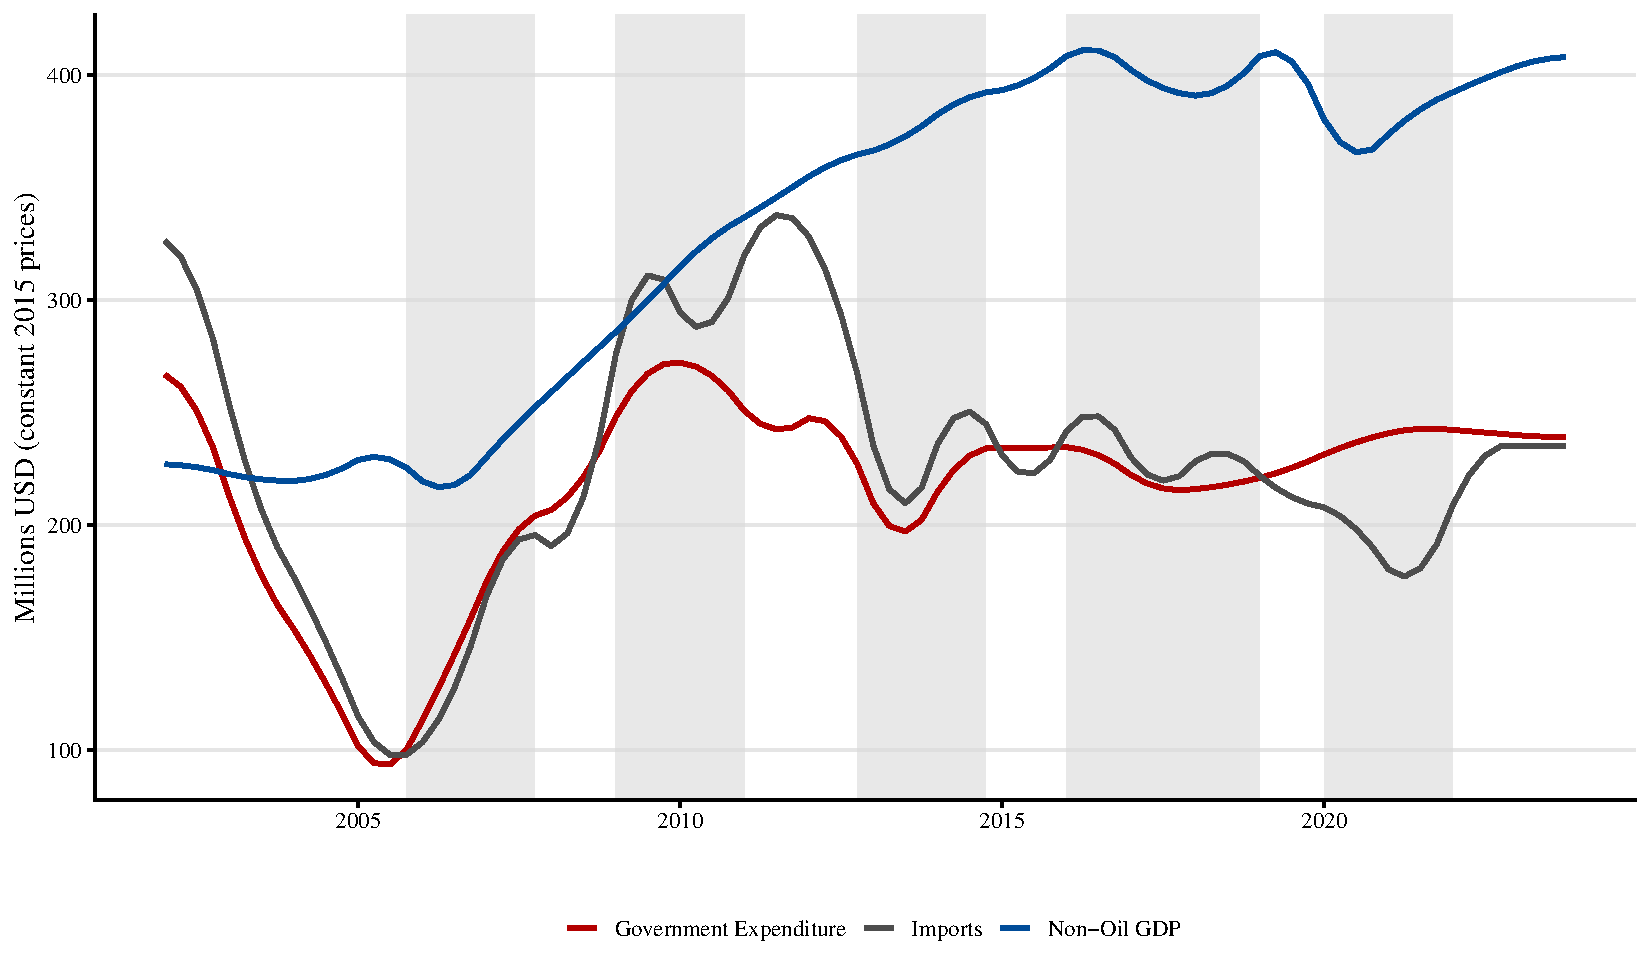
\includegraphics[width=\textwidth]{../graphics/figure_1_macro_levels_long.pdf}
  \caption{Levels}
\end{subfigure}\hfill
\begin{subfigure}[t]{0.49\textwidth}
  \centering
  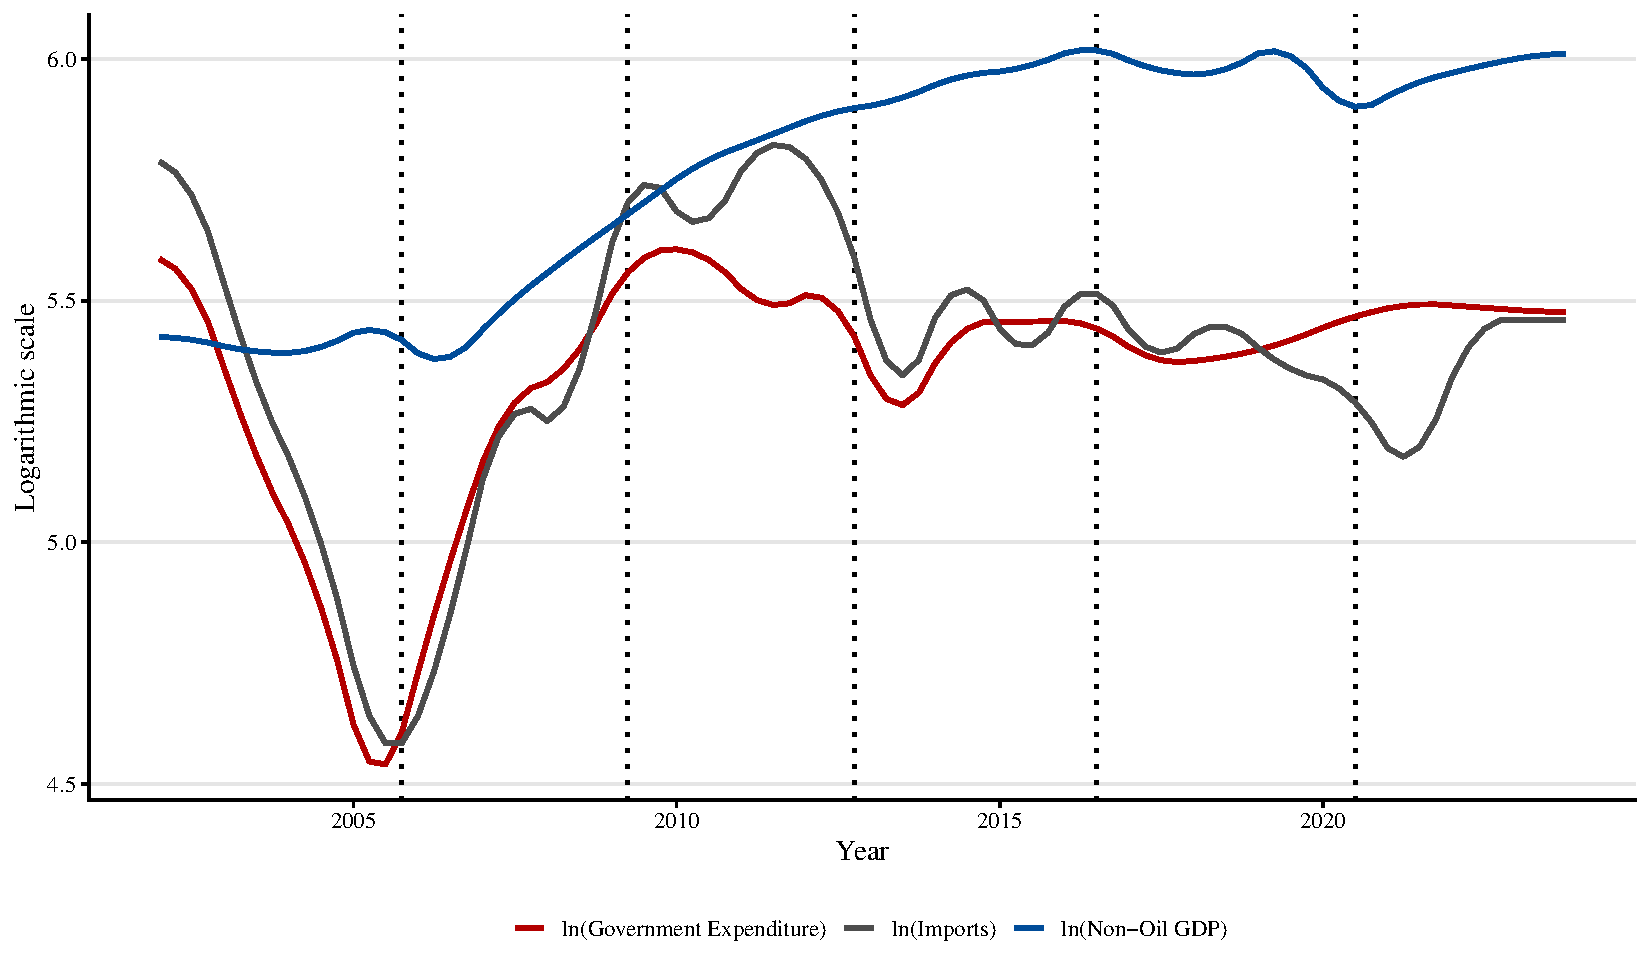
\includegraphics[width=\textwidth]{../graphics/figure_2_macro_log_long.pdf}
  \caption{Logarithms and breaks}
\end{subfigure}
\caption{Long-sample macroeconomic series, 2002Q1--2023Q4. Gray areas mark event windows; dotted lines mark the main breaks selected by BIC across the five series. Source: Author's elaboration.}
\label{fig:macro_long}
\end{figure}

\begin{table}[htbp]
\centering
\small
\caption{Unit-root and stationarity tests, long sample}
\label{tab:stationarity_long}
\begin{tabular}{@{}lcccccl@{}}
\toprule
Series & ADF ($p$) & KPSS ($p$) & ZA ($t$) & 5\% CV & Break & Stationary? \\
\midrule
\texttt{ln\_gov\_exp} & 0.085 & 0.016 & $-5.09$ & $-5.08$ & 2005Q1 & Yes \\
\texttt{ln\_gdp\_non} & 0.943 & 0.010 & $-3.37$ & $-5.08$ & 2007Q2 & No \\
\texttt{ln\_imports} & 0.381 & 0.100 & $-3.68$ & $-5.08$ & 2008Q1 & No \\
\texttt{ln\_cpi} & 0.599 & 0.010 & $-4.02$ & $-5.08$ & 2009Q4 & No \\
\texttt{ln\_credit} & 0.010 & 0.010 & $-12.66$ & $-5.08$ & 2003Q1 & Yes \\
\bottomrule
\end{tabular}
\par\vspace{0.3em}
\begin{minipage}{0.95\textwidth}
\footnotesize\textit{Note:} See the notes to Table~\ref{tab:stationarity}. Source: Author's elaboration.
\end{minipage}
\end{table}

\section{Additional results}
\label{sec:appendix_results}

Figure~\ref{fig:stability_official} shows the companion roots for the official three-variable model. All roots lie inside the unit circle. Figure~\ref{fig:fevd} compares the FEVDs of the official and long three-variable models. Figures~\ref{fig:irf_full_official} and~\ref{fig:irf_full_long} present the complete IRF matrices for the official and long three-variable models.

\begin{figure}[htbp]
\centering
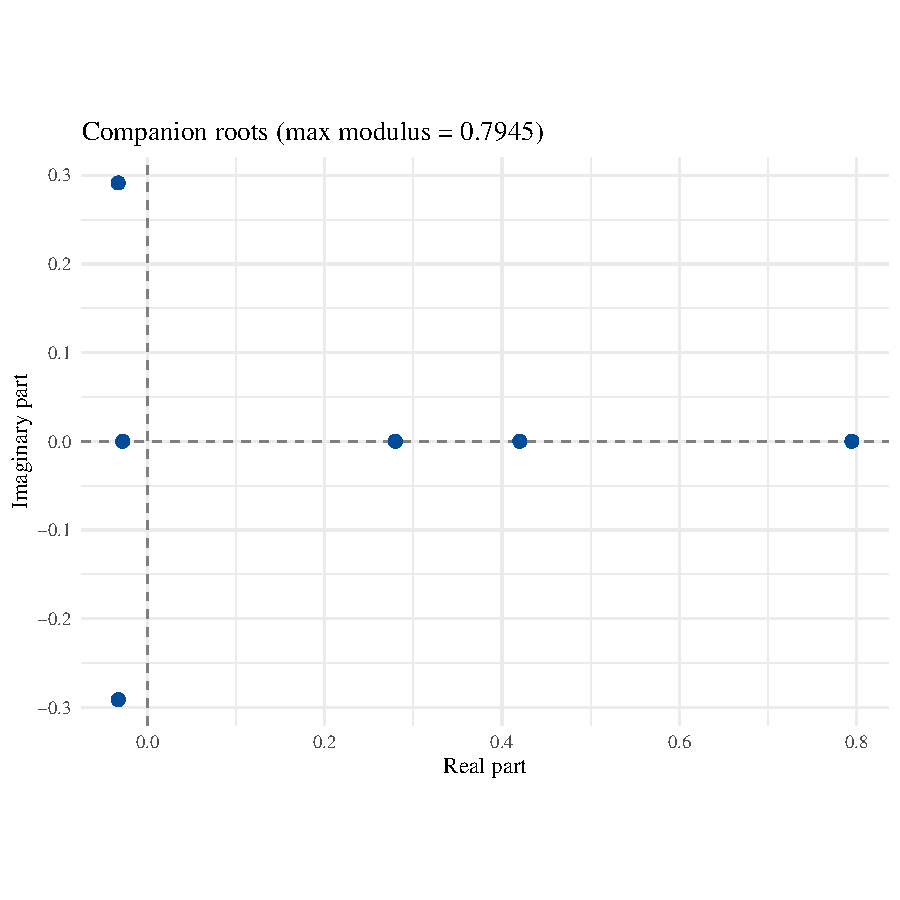
\includegraphics[width=0.55\textwidth]{../graphics/stability_roots_order_1_official_3var.pdf}
\caption{Companion roots of the official three-variable BVAR. The maximum modulus is 0.795, below one. Source: Author's elaboration.}
\label{fig:stability_official}
\end{figure}

\begin{figure}[htbp]
\centering
\begin{subfigure}[t]{0.49\textwidth}
  \centering
  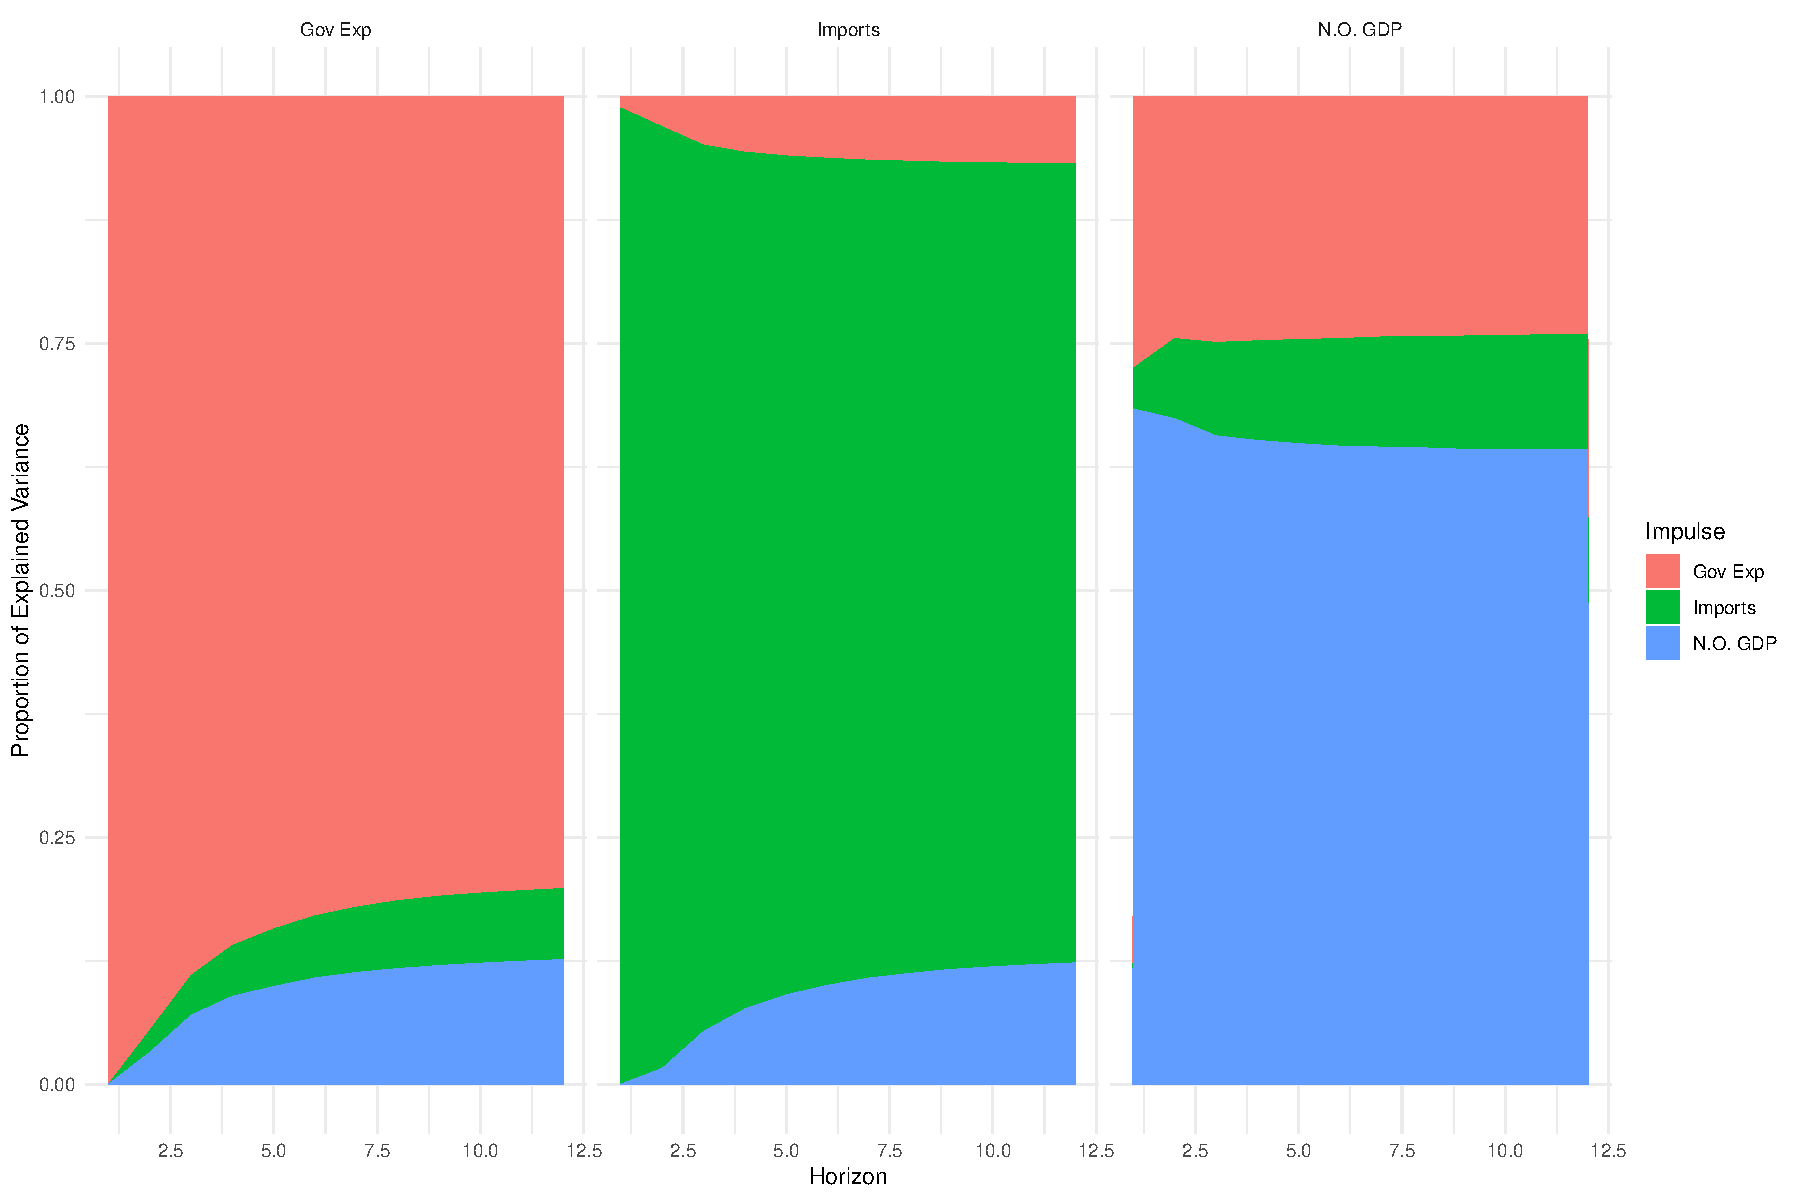
\includegraphics[width=\textwidth]{../graphics/fevd_median_order_1_official_3var.pdf}
  \caption{Official sample}
\end{subfigure}\hfill
\begin{subfigure}[t]{0.49\textwidth}
  \centering
  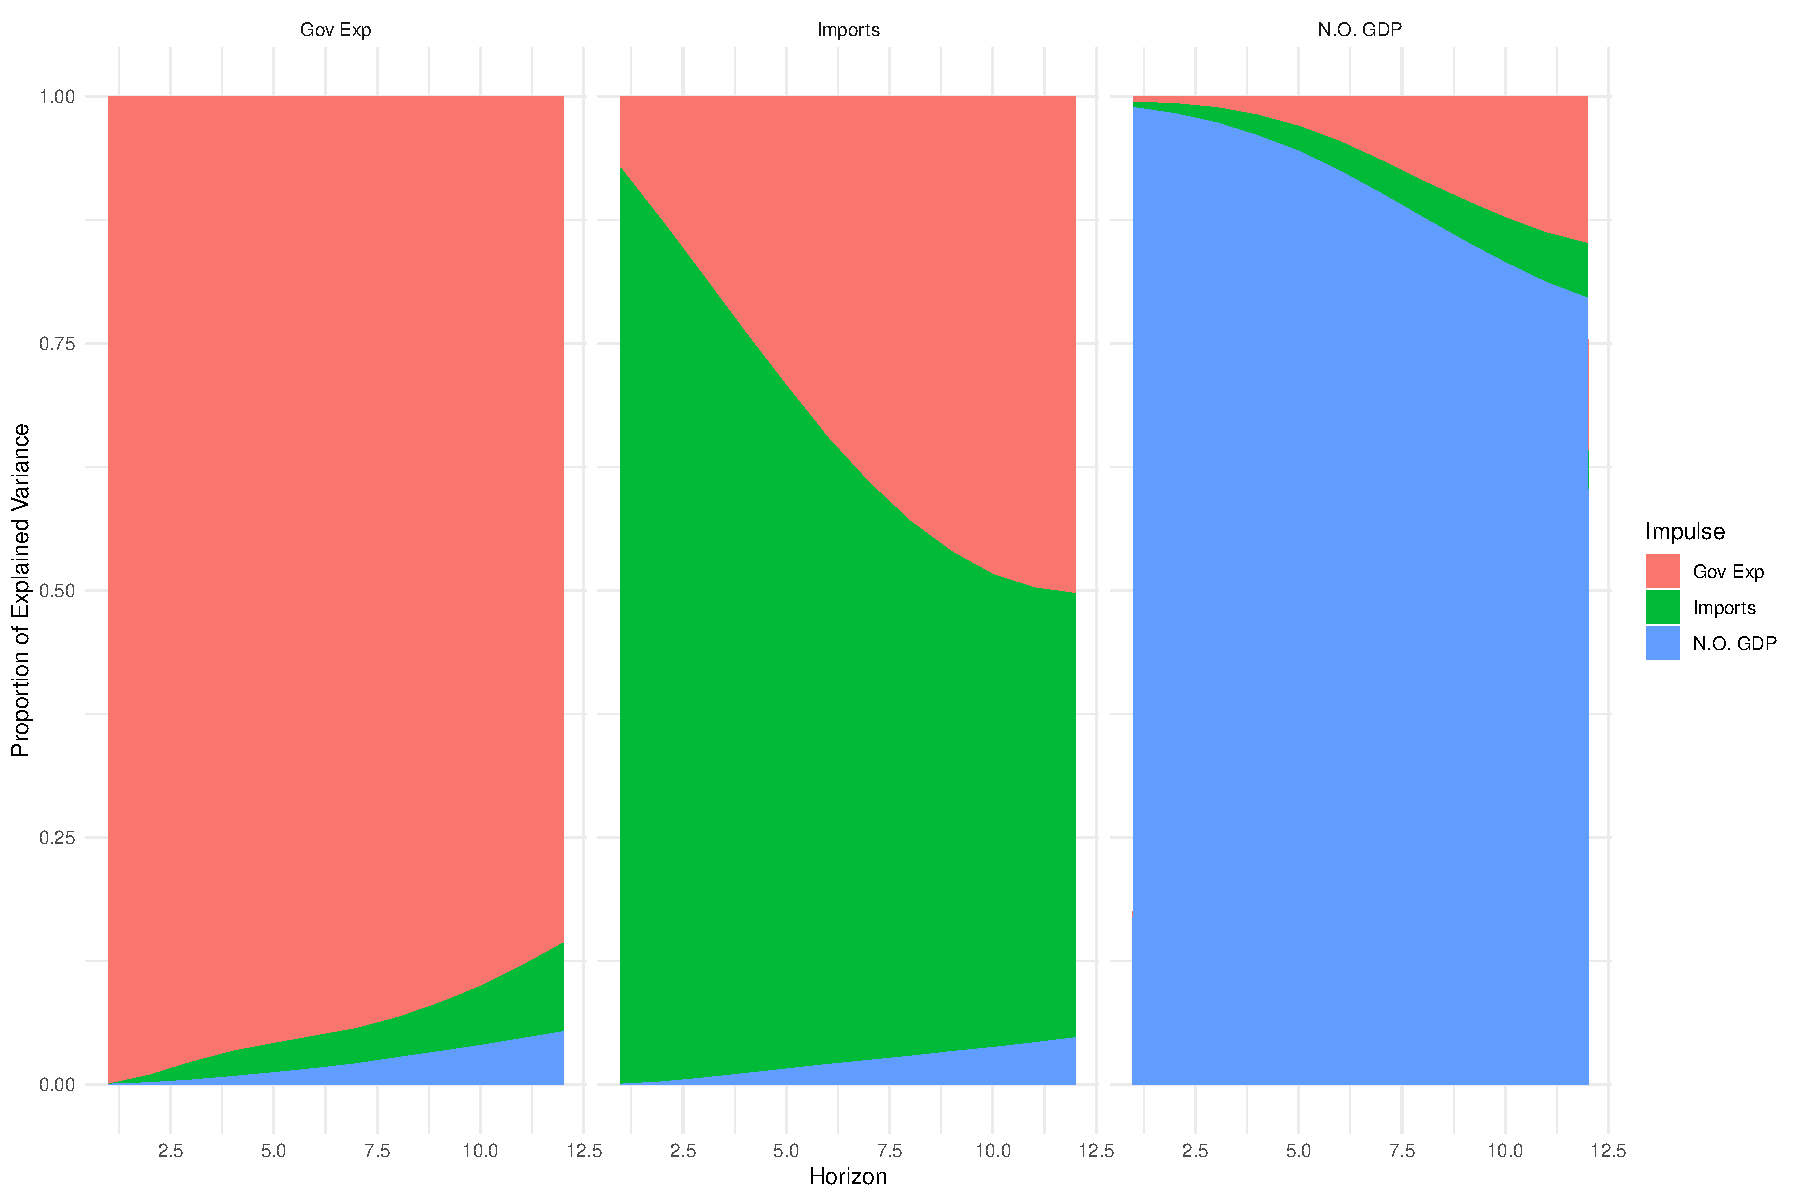
\includegraphics[width=\textwidth]{../graphics/fevd_median_order_1_long_3var.pdf}
  \caption{Long sample}
\end{subfigure}
\caption{Forecast-error variance decomposition, three-variable BVAR, order 1. Source: Author's elaboration.}
\label{fig:fevd}
\end{figure}

\begin{figure}[p]
\centering
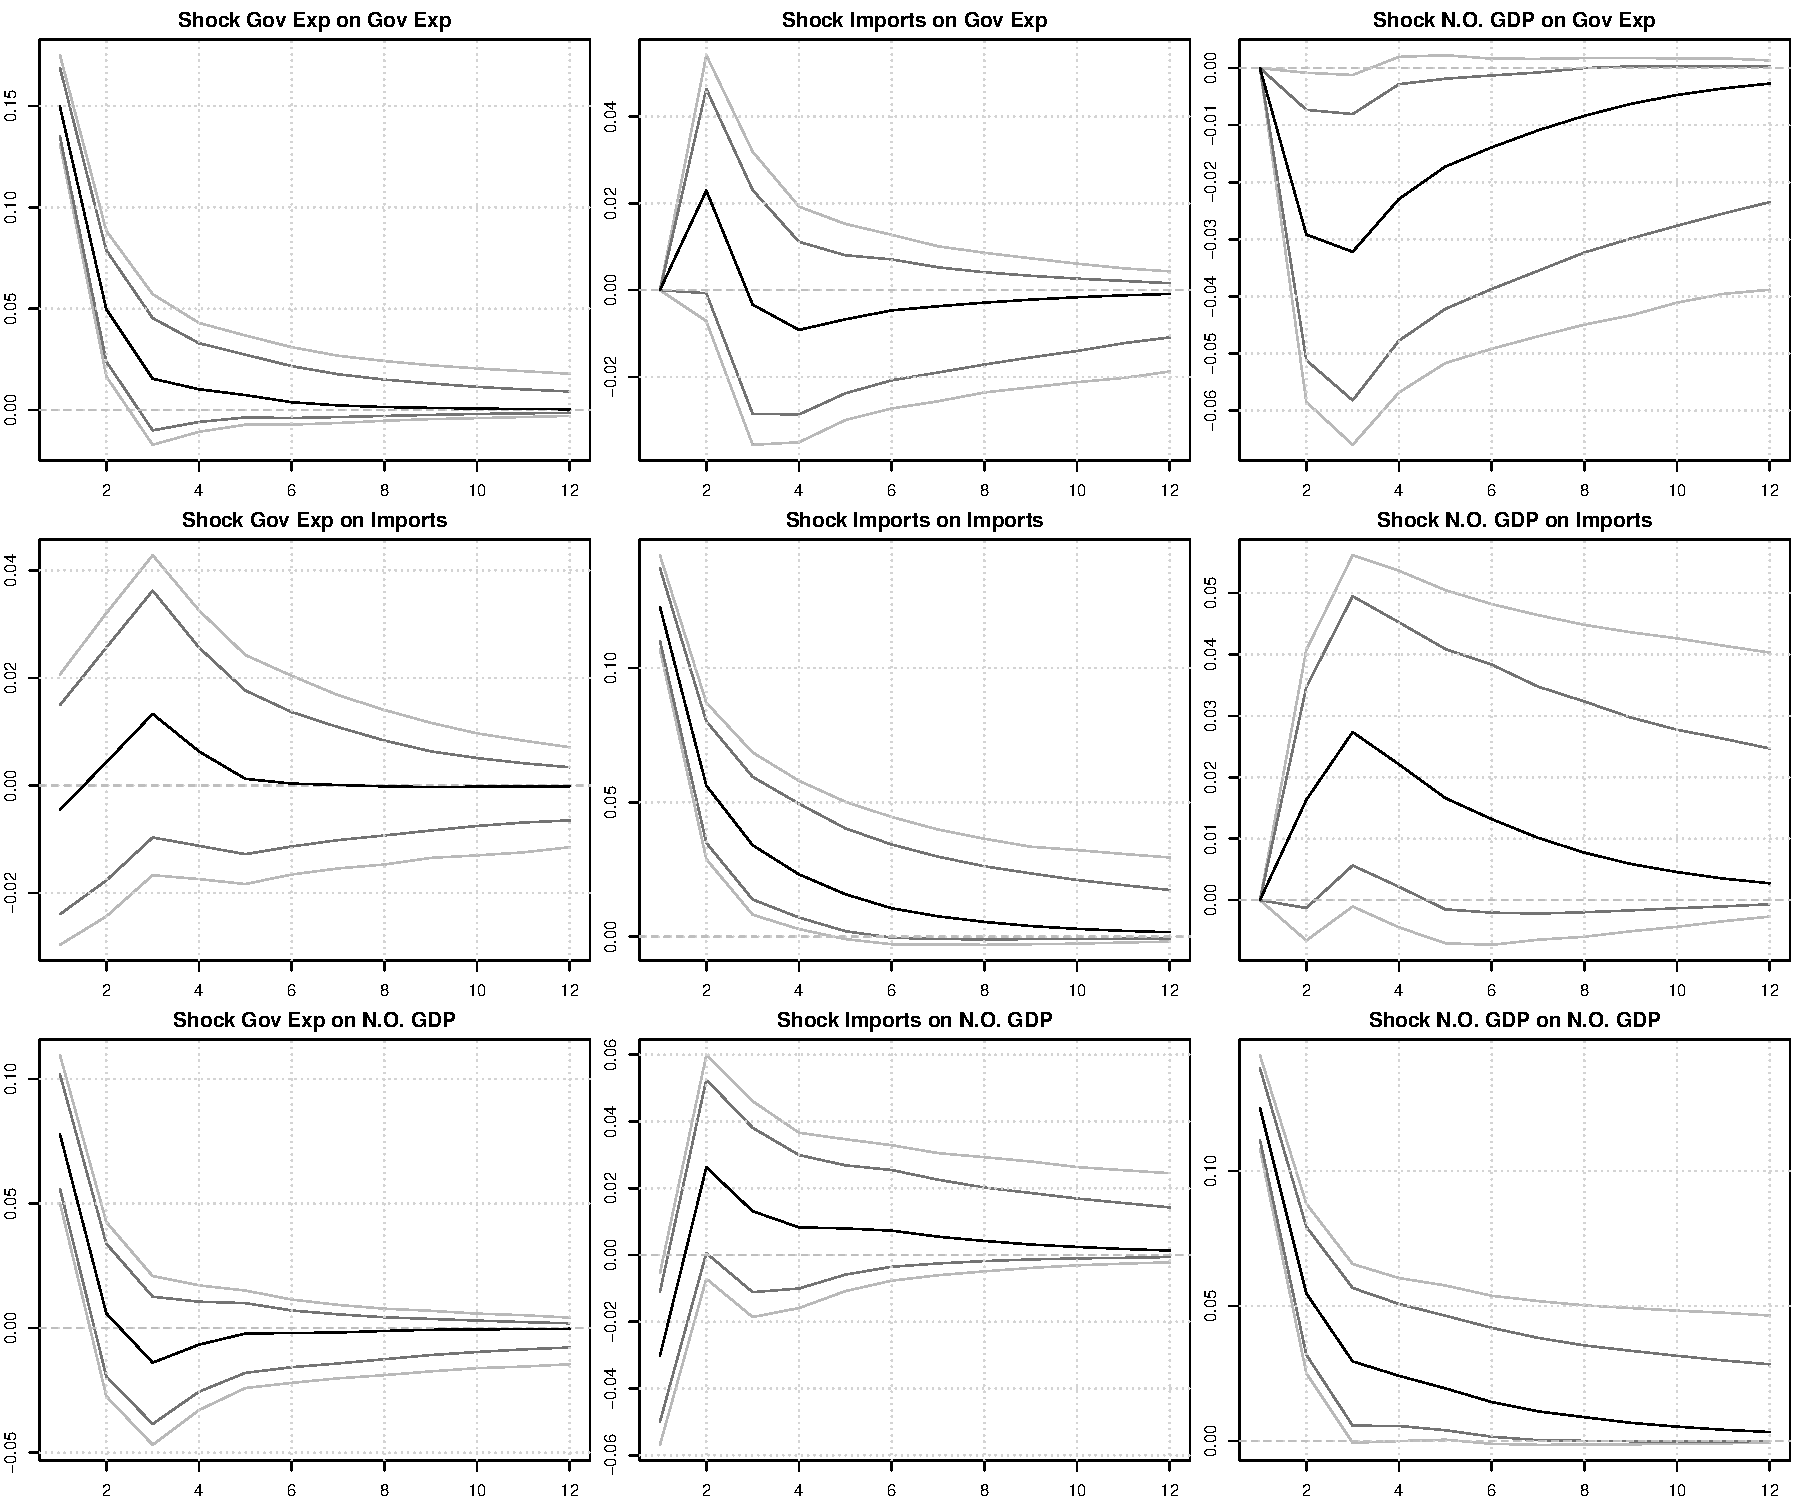
\includegraphics[width=0.95\textwidth]{../graphics/irf_full_matrix_order_1_official_3var.pdf}
\caption{Complete matrix of orthogonalized IRFs, official sample, order 1. Each panel shows the response of the variable after ``on'' to a shock to the variable after ``Shock''. Bands: 68\% and 90\%. Source: Author's elaboration.}
\label{fig:irf_full_official}
\end{figure}

\begin{figure}[p]
\centering
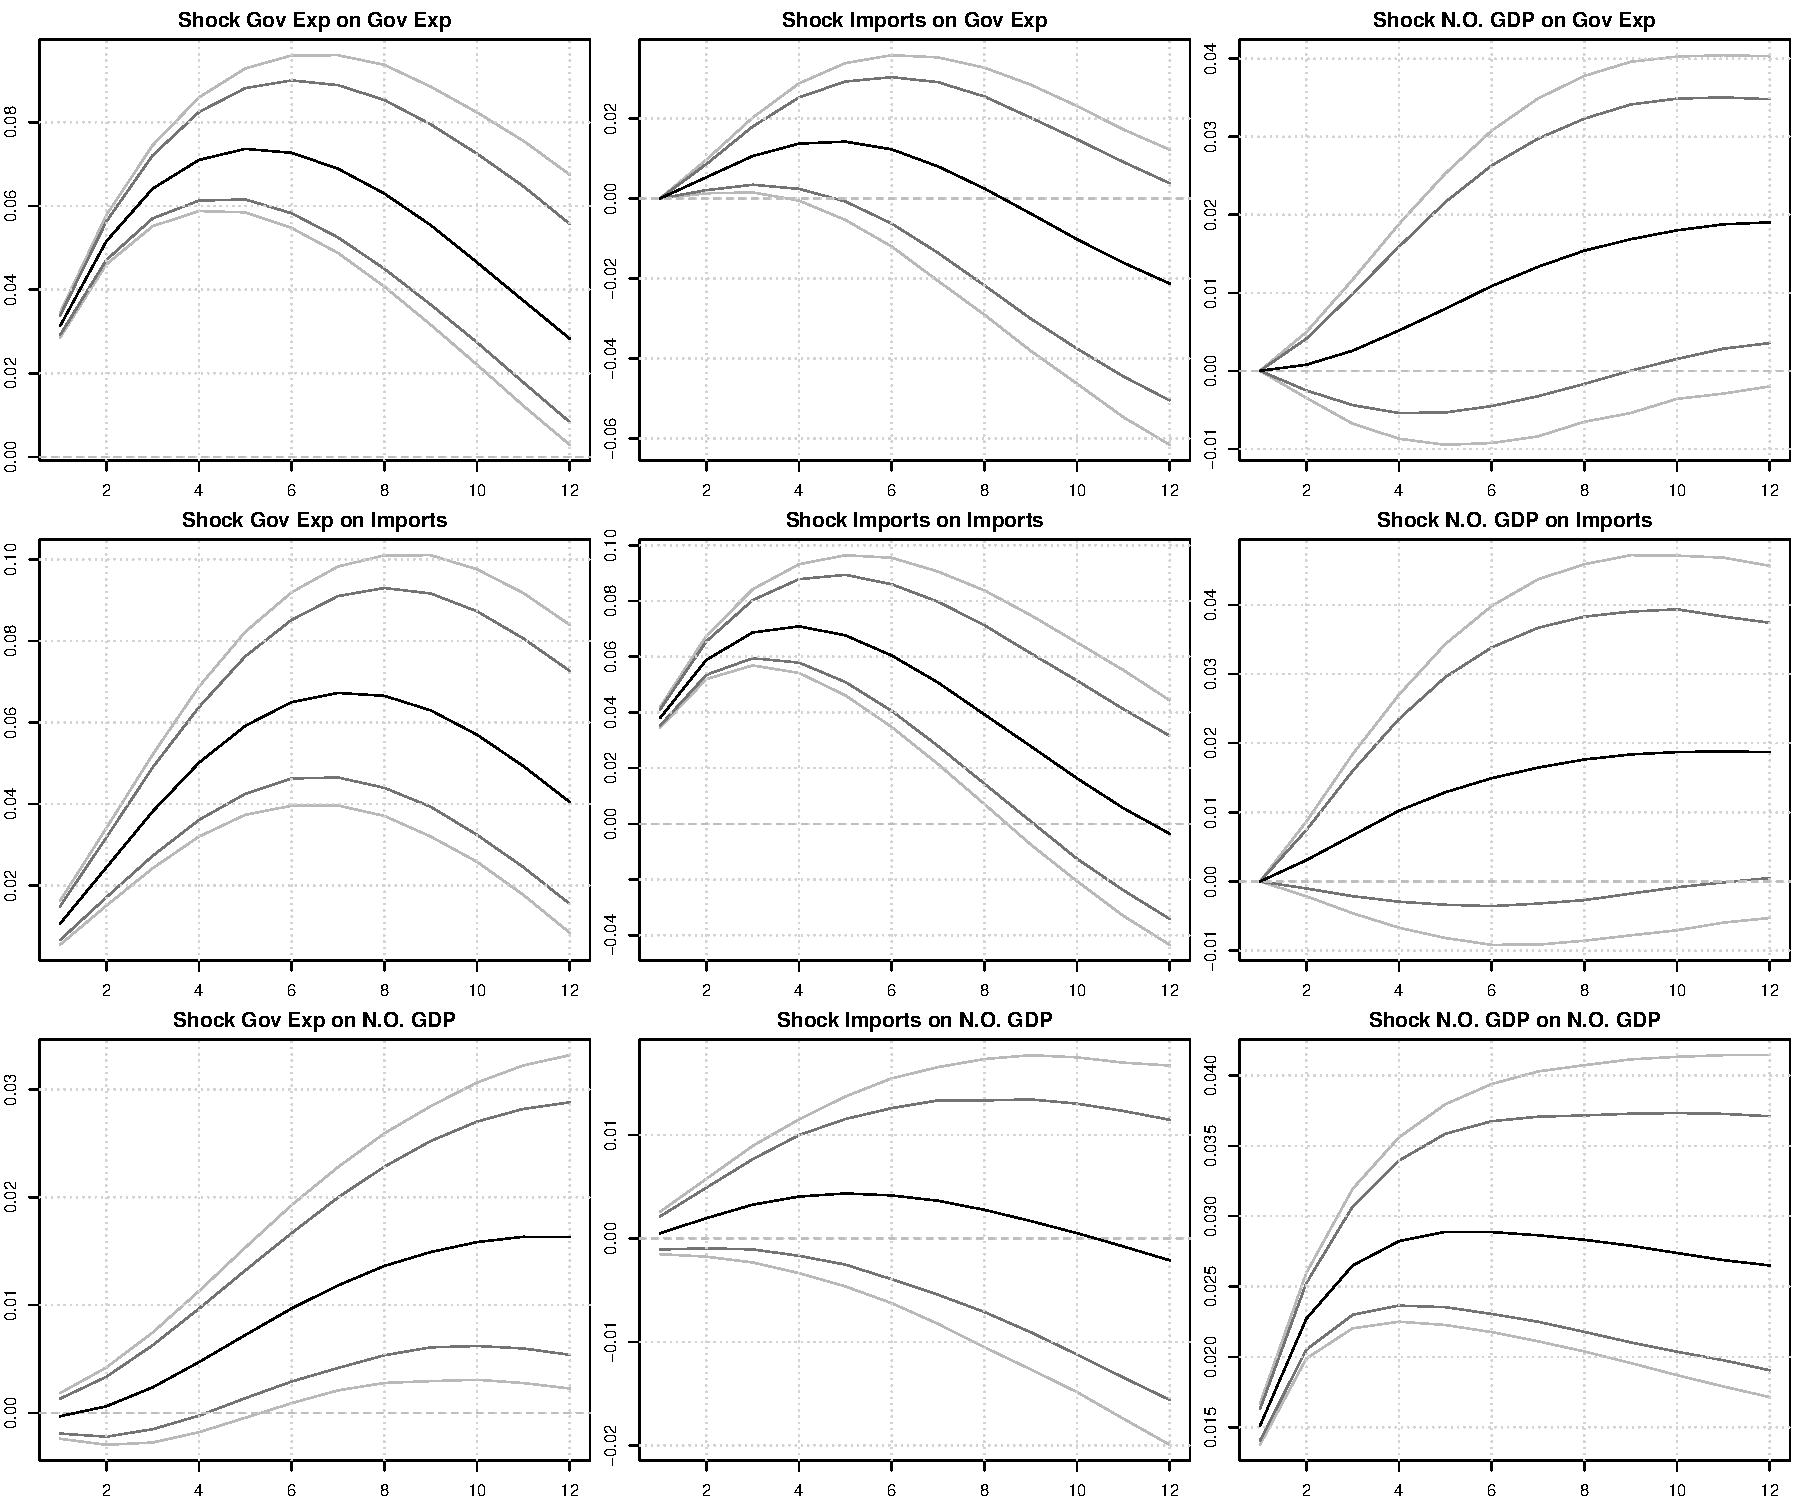
\includegraphics[width=0.95\textwidth]{../graphics/irf_full_matrix_order_1_long_3var.pdf}
\caption{Complete matrix of orthogonalized IRFs, long sample, order 1. Each panel shows the response of the variable after ``on'' to a shock to the variable after ``Shock''. Bands: 68\% and 90\%. Source: Author's elaboration.}
\label{fig:irf_full_long}
\end{figure}

\end{document}
